\documentclass[12pt,bibliography=oldstyle,DIV=12,parskip=half-]{scrreprt}
% esto me setea la variable pdf dependiendo del valor de \pdfoutput, que es >0
% sólo cuando estoy usando pdflatex para compilar el documento
%% \newif\ifpdf
%% \ifnum\pdfoutput<0
%% \pdffalse\fi
%% \ifnum\pdfoutput=0
%% \pdffalse\fi
%% \ifnum\pdfoutput>0
%% \pdftrue\fi


%
% ===
% === Trick para detectar si el documento está siendo compilado con pdflatex
% ===
%
% Esto me setea la variable pdf dependiendo del valor de \pdfoutput, que es >0
% sólo cuando estoy usando pdflatex para compilar el documento. Con esto puedo
% hacer  \ifpdf {...} \fi, que se ejecuta colo cuando compilo con pdflatex.
%% \newif\ifpdf
%% \ifnum\pdfoutput<0
%% \pdffalse\fi
%% \ifnum\pdfoutput=0
%% \pdffalse\fi
%% \ifnum\pdfoutput>0
%% \pdftrue\fi
%
% ===
% === I18n / L10n
% ===
%
% babel me da separación de sílabas para palabras en el idioma que le paso como
%       argumento opcional.
\usepackage[spanish,es-tabla,english]{babel}
%
% inputenc define la codificación de caracteres del código fuente, acá utf8.
\usepackage[utf8]{inputenc}
%
% ===
% === Gráficos
% ===
% 
% pst-pdf me permite usar PSTricks con pdflatex. Necesito cargarlo sólo si está
%         definida la variable pdf, por eso está entre \ifpdf ... \fi
%\ifpdf\usepackage{pst-pdf}\fi
%
% color me permite usar colores en el documento.
\usepackage{color}
%
% graphicx me da el comando \includegraphics para insertar imágenes (?)
\usepackage{graphicx}
%
% pstricks es un conjunto de macros basadas en PostScript para TeX, en
%          castellano: me da un entorno pstricks y comandos que uso dentro de
%          éste, que me sirven para dibujar figuras/diagramas/etc de manera
%          relativamente simple.
%\usepackage{pstricks}
%
% pst-circ me da macros para pstricks que me dibujan elementos de circuitos
%\usepackage{pst-circ}
%
% pst-plot me provee de funciones de ploteo para pstricks
%\usepackage{pst-plot}
%
% pst-2dplot me sirve para plotear en pstricks, entorno pstaxes
%\usepackage{pst-2dplot}
%
% ===
% === Verbatims
% ===
%
% verbatim es una reimplementación de los entornos verbatim[*]
%          provee el comando \verbatiminput{archivo} y el entorno comment, que
%          hace que LaTeX ignore directamente todo lo que está adentro
%\usepackage{verbatim}
%
% moreverb implementa el entorno verbatimtab indentando los tabs que encuentre,
%          y también el entorno listing, que pone números de línea al verbatim.
%          Para cambiar el ancho de la tabulacion, uso
%          \renewcommand\verbatimtabsize{<ancho del tab>\relax}
%          También define el entorno boxedverbatim.
%\usepackage{moreverb}
%
% listings me da el entorno lstlisting con resaltado de sintaxis.
%          Para setear el lenguaje del código, hago \lstset{language=<lang>}
%\usepackage{listings}
%
% url es un verbatim para escribir URL's que permite linebreaks dentro de ésta.
%     para usarlo, \url{<URL>}
\usepackage{url}
%
% ===
% === Más packages
% ===
%
%% \usepackage{mdwlist}		%Para listas mas compactas
%% \usepackage{textcomp}		%Para algunos símbolos
%% \usepackage{colortbl}		%Para celdas de colores en tablas
%% \usepackage{fancyhdr}		%Para encabezados/pie
\usepackage{bbold}		%Fuente bb para modo math: \mathbb{R} = reales
\usepackage{dsfont}		%Fuente ds para modo math: \mathds{R} = reales
\usepackage{multirow}		%Para "combinar" celdas en tablas
\usepackage{float}		%Para mejorar cuadros, figuras, etc
%% \usepackage{fancybox}		%Para recuardos de texto con bordes "fancy"
%% \usepackage{dingbat}		%Para dingbats
%\usepackage{marginal}		%Para  notas al margen que no puedo hacer andar
\usepackage{amsmath}		%Para enornos matemáticos mas flexibles
%\usepackage{varwidth}		%varwidth es un minipage que se ajusta al ancho mínimo


\usepackage[backend=biber,sorting=none,style=ieee,eprint=false,url=false]{biblatex} %% style=ieee
%% requiere texlive-bibtex-extra en debian


\usepackage{enumitem}
\setlist{noitemsep}
%% \setlist[description]{noitemsep}
%% \setlist[enumerate]{noitemsep}
%% \setlist[itemize]{noitemsep}

\usepackage{tikz}
\usepackage{pgfkeys}
\usepackage{pgfgantt}

% typearea: uso con koma-script para ajustar márgenes de página.
% vars globales a setear en la clase koma-script: DIV=12, BCOR=margen de ``binding'' para double side
\usepackage{typearea}

% para poder usar footnotes p.ej, adentro de un tabular
\usepackage{footnote}
\makesavenoteenv{tabular}

% para tabulars mas lindos/legibles
\usepackage{booktabs}

%\usepackage{glossaries}

\usepackage[spanish]{algorithm2e}

% para highlight (comando \hl{})
\usepackage{soulutf8}

% para teoremans etc
\usepackage{amsthm}

% para tunear citations
%\usepackage[square,comma,numbers,sort&compress]{natbib}


% config.tex: configuraciones del documento
%\selectlanguage{spanish}		%Elijo idioma español

%Permitir que los entornos equation, align, etc permitan saltos de página
%\allowdisplaybreaks[1]

%Tweaks
%% \setlength{\parindent}{0mm}		%Sangría de 1a. línea
%% \setlength{\hoffset}{2.6mm}		%
%% \setlength{\voffset}{-5.4mm}		%
%% \setlength{\topmargin}{0mm}		%
%% \setlength{\oddsidemargin}{5mm}	%
%% \setlength{\evensidemargin}{5mm}	%
%% \setlength{\marginparsep}{5mm}	%
%% \setlength{\headheight}{12.5mm}	%
%% \setlength{\headsep}{2.5mm}		%
%% \setlength{\footskip}{10mm}		%
%% \setlength{\textwidth}{14.1cm}		%
%% \setlength{\textheight}{232mm}	%
%% \setlength{\fboxrule}{.1pt}
%% \setlength{\parskip}{.5\baselineskip}

%Colores
\definecolor{negro}	{cmyk}{0,0,0,1}
\definecolor{marron}	{cmyk}{0,.5,1,.41}
\definecolor{rojo}	{cmyk}{0,1,1,0}
\definecolor{naranja}	{cmyk}{0,.35,1,0}
\definecolor{amarillo}	{cmyk}{0,0,1,0}
\definecolor{verde}	{cmyk}{1,0,1,0}
\definecolor{azul}	{cmyk}{1,1,0,0}
\definecolor{violeta}	{cmyk}{.45,1,0,0}
\definecolor{gris}	{cmyk}{0,0,0,.5}
\definecolor{blanco}	{cmyk}{0,0,0,0}
\definecolor{dorado}	{cmyk}{0,.16,1,0}
\definecolor{plateado}	{cmyk}{0,0,0,.25}

%% \title{\titulo}
%% \author{\autor}
%% \date{\fecha}

% si uso pdflatex, me setea las propiedades del pdf de salida
%% \ifpdf\pdfinfo{/Title    (\tituloPDF)
%%                /Author   (\autorPDF)
%%                /Subject  (\asuntoPDF)
%%                /Keywords (\clavesPDF)}\fi

% comandos.tex
% en este archivo defino todos los comandos/environment que quiera usar en mi documento.
%
% ===
% === Comandos
% ===
% 
% T: para escribir texto común cuando en modo math
%    uso: \T{texto que aparecerá en letra normal}
\newcommand{\T}{\textrm}
%
% aclaracion: dibuja un recuadrito aclaratorio, como <quote> en HTML.
%             uso: \aclaracion{Texto...}
\newcommand{\aclaracion}[1]{%
\smallpencil\-\begin{minipage}{0.9\textwidth}
%\vspace*{6pt}
{#1}\smallskip\end{minipage}}
%
% consigna: parecido a aclaración, pero con texto _slanted_
%           uso: \consigna{Consigna...}
\newcommand{\consigna}[1]{%
\leftpointright\ \parbox[t]{0.9\textwidth}{\textsl{#1}\vspace{8pt}}}
%
% pinterno: para representar el producto interno entre los dos argumentos
%           uso: \pinterno{X}{Y}
\newcommand{\pinterno}[2]{%
\left\langle #1 , #2 \right\rangle}
%
% === Estilos de texto
%
% resalt: resaltado con fondo verde
%         uso: \resalt{texto resaltado}
\newcommand{\resalt}{\colorbox{yellow}}
%
% sfbf: texto en negrita + slanted
%       uso:
\newcommand{\sfbf}[1]{\textsf{\bfseries #1}}
%
% small bold sans-serif
\newcommand{\sbs}[1]{\textsf{\small\bfseries #1}}
%
% eng: itálica (para palabras en inglés)
%      uso: \eng{some English text}
\newcommand{\eng}{\textit}
%
% mean: significado de una sigla - slanted
%       uso: (...) SNCF: \mean{Société Nationale des Chemins de Fer Francais} ...
\newcommand{\mean}{\textsl}
\newcommand{\desc}{\textsl}
%
% defin: pone en negrita el texto, útil para definiciones
%        uso: \defin{asshole}: vulgar slang for anus
\newcommand{\defin}{\textbf}
%
% R, N: cambia la tipografía en modo math, probar para ver cómo quedan
%       uso: \R{R} , \N{N}
\newcommand{\R}{\mathds}
\newcommand{\N}{\mathbf}
\newcommand{\C}{\mathcal}
\newcommand{\B}{\boldsymbol}
%
% dx: para escribir d2y/dx2, etc
\newcommand{\dx}[2]{\frac{d^{#2}\!#1}{d\!x^{#2}}}
%
% dp: para escribir derivadas parciales d2y/dx2, etc
\newcommand{\dpar}[3]{\frac{\partial^{#3}#1}{\partial{#2}^{#3}}}
%
% dvar: para escribir derivadas totales d2y/d(VAR)2, etc
\newcommand{\dvar}[3]{\frac{d^{#3}#1}{d{#2}^{#3}}}
%
% evalen: para escribir (loquesea)|_{evaluado_en}
\newcommand{\evalen}[2]{\left.{#2}\right|_{#1}}
%
% lil: para escribir texto pequeño. más cómodo que { \footnotesize texto pequeño... }
%      uso: \lil{texto pequeño... }
\newcommand{\lil}[1]{\footnotesize #1}  %Para texto pequeñooo
%
% mono: escribe el texto que le paso como parámetro con letra de ancho fijo
%       uso: \mono{texto monoespaciado}
\newcommand{\mono}[1]{{\texttt{#1}}}
%
% === Símbolos
%
\newcommand{\y}{\wedge}			%Y (Lógica)
\newcommand{\ve}{\vee}			%O (Lógica)
\newcommand{\ent}{\supset}		%Entonces (Lógica)
\newcommand{\dimp}{\leftrightarrow}	%Doble implicativo, equivalencia (Lógica)
\newcommand{\sii}{\leftrightarrow}	%Si y sólo si (Lógica)
\newcommand{\equi}{\equiv}		%Equivalencia (Lógica)
\newcommand{\portanto}{\vdash}		%Por lo tanto (Lógica)
\newcommand{\por}{\cdot}		%Producto punto
\newcommand{\RR}[1][1]{\mathds{R}}	%R de reales
\newcommand{\hfi}{\hat{\phi}}           %fi con gorrito arriba
\newcommand{\bfi}{\bar{\phi}}           %fi con raya arriba
\newcommand{\hpsi}{\hat{\psi}}          %Letra griega psi con gorrito arriba
\newcommand{\II}{\B{I}}                 %w negrita
\newcommand{\KK}{\B{K}}                 %w negrita
\newcommand{\QQ}{\B{Q}}                 %w negrita
\newcommand{\YY}{\B{Y}}                 %w negrita
\newcommand{\Bg}{\B{g}}                 %w negrita
\newcommand{\nn}{\B{n}}                 %w negrita
\newcommand{\uu}{\B{u}}                 %w negrita
\newcommand{\vv}{\B{v}}                 %w negrita
\newcommand{\ww}{\B{w}}                 %w negrita
\newcommand{\xx}{\B{x}}                 %x negrita
\newcommand{\yy}{\B{y}}                 %y negrita
\newcommand{\zz}{\B{z}}                 %z negrita
\newcommand{\BPhi}{\B{\Phi}}            %\Phi negrita
\newcommand{\Balpha}{\B{\alpha}}        %\alpha negrita
\newcommand{\Bbeta}{\B{\beta}}          %\beta negrita
\newcommand{\Btheta}{\B{\theta}}        %\theta negrita
\newcommand{\Bxi}{\B{\xi}}              %\xi negrita
%
%
% ===
% === Environments
% ===
% 
% enunciado: un environment que básicamente tiene el mismo efecto que el
%            comando consigna.
%            uso: \begin{enunciado} ... contenido ... \end{enunciado}
\newenvironment{enunciado}
{\leftpointright\ \begin{varwidth}[t]{0.9\textwidth}\textsl}
{\end{varwidth}\vspace{8pt}}
%
% pvi: para tipear la definición de un problema de valor inicial/funciones
%      definidas de a trozos/etc directamente en el texto (sin necesidad de
%      cambiar a un modo matemático.
%      uso: \begin{pvi} linea1 \\ linea 2 \\ ... \end{pvi}
\newenvironment{pvi}{\begin{equation}\begin{cases}}
{\end{cases}\end{equation}}
%
% pvi*: comp pvi, pero sin número de ecuación
\newenvironment{pvi*}{\begin{equation*}\begin{cases}}
{\end{cases}\end{equation*}}
%
% verbatimsmall: un verbatim con letra más chica. usualmente queda bastante
%                mejor que el verbatim pelado.
%                uso: \begin{verbatimsmall} ........ \end{verbatimsmall}
\newenvironment{verbatimsmall}{\small\begin{verbatim*}}
{\end{verbatim*}}
%
% nota: escribe una aclaracion dentro del texto
\newenvironment{nota}{$$\left[\;\begin{minipage}{0.95\textwidth}\slshape}
{\end{minipage}\;\right]$$}
%
%
% ===
% === Comandos ``históricos''
% ===
%
%% %\begin{pspicture}
%% \def\tierra(#1){%Para dibujar el símbolo de tierra en el entorno PSTricks
%% 	\rput(#1){
%% 		\psdot(0,0)
%% 		\psline(0,0)(0,-0.45)
%% 		\psline(-0.5,-0.45)(0.5,-0.45)
%% 		\psline(-0.35,-0.6)(0.35,-0.6)
%% 		\psline(-0.2,-0.75)(0.2,-0.75)
%% 	}%
%% }
%% %\end{pspicture}

\newcommand{\codigo}[2]{%Para generar un recuadro con código
	%\setlength{\hrulewidth}{0.1pt}
	\begin{flushleft}
	\underline{#1}
	\begin{tabular}{@{\quad}|l}
		\begin{minipage}{.85\textwidth}\smallskip{#2}
	\end{minipage}\end{tabular}\end{flushleft}%
}

\newcommand{\filecodigo}[1]{%Insertar código verbatim desde un archivo
\codigo{#1}{\verbatiminput{#1}}}%Requiere el paquete verbatim
\newcommand{\filecodigobis}[1]{{\verbatiminput{#1}}}%Requiere el paquete verbatim

%% \newcommand{\grafico}[3][1]{%Para generar un plot de un archivo con coords.
%% %\def\deequis=#1
%% \begin{minipage}{0.5\textwidth}\begin{center}
%% \begin{pspicture}(6,5)
%% 	\psgrid[subgriddiv=1,gridlabels=0pt,gridwidth=.1pt](1,3)(1,1)(6,5)
%% 	\psset{xunit=5cm,yunit=2cm}
%% 	\fileplot[linewidth=1pt,linecolor=blue,origin={0.2,1.5}]{#2}
%% 	\psset{xunit=1cm,yunit=1cm}
%% 	\psaxes[Dx=#1,dx=5,Oy=-1,Dy=1,dy=2]{-}(0.9,1)(6,5)
%% 	\rput(4,0.4){\textsl{#3}}
%% \end{pspicture}\end{center}\end{minipage}}

%% \newcommand{\eqncode}[2]{%
%% \begin{center}
%% \begin{tabular}{l@{\hspace{0.5cm}}r}
%% \begin{minipage}{.4\textwidth}
%% \begin{equation*}
%% #1
%% \end{equation*}
%% \end{minipage}
%% &
%% \fbox{\begin{minipage}{.4\textwidth}
%% %\setlength{\parskip}{4mm}
%% \filecodigobis{#2}
%% \end{minipage}}
%% \end{tabular}
%% \end{center}
%% }

%% \newcommand{\eqncodeb}[2]{%
%% \begin{center}\begin{tabular}{l@{\hspace{0.5cm}}r}
%% \begin{minipage}{.4\textwidth}#1\end{minipage} &
%% \fbox{\begin{minipage}{.4\textwidth}\filecodigobis{#2}\end{minipage}}
%% \end{tabular}\end{center}}

%% \newenvironment{matemcode}[1]{\newline
%% \begin{tabular}{l@{\hspace{0.5cm}}r}
%% \begin{minipage}{.4\textwidth}
%% \parbox[t]{.4\textwidth}{\begin{equation*}#1\end{equation*}}\end{minipage}
%% &\begin{Sbox}\begin{minipage}{.4\textwidth}}
%% {\end{minipage}\end{Sbox}\fbox{\TheSbox}\end{tabular}\newline}

%% \newenvironment{encuadrar}[1]{\begin{Sbox}\begin{varwidth}{#1\textwidth}}
%% {\end{varwidth}\end{Sbox}\fbox{\TheSbox}}

%% \newenvironment{parboxenv}{\begin{Sbox}}
%% {\end{Sbox}\parbox[t]{.9\textwidth}{\TheSbox}}

% multicolumn y multirow
\newcommand{\mcol}[3]{\multicolumn{#1}{#2}{#3}}
\newcommand{\mrow}[3]{\multirow{#1}{#2}{#3}}

%% Serif .......................................................................
%%
%% New Century Schoolbook
%% \usepackage[T1]{fontenc}
%% \usepackage{fouriernc}
%%
%%
%% TeX Gyre Schola (New Century extendida)
%% \usepackage[T1]{fontenc}
%% \usepackage{tgschola}
%%
%%
%% Utopia
%% \usepackage[T1]{fontenc}
%% \usepackage{fourier}
%%
%%
%% Utopia (con MathDesign)
%% \usepackage[T1]{fontenc}
%% \usepackage[adobe-utopia]{mathdesign}
%%
%%
%% Computer Concrete
%% \usepackage[T1]{fontenc}
%% \usepackage{concmath}
%%
%%
%% Charter BT
 \usepackage[T1]{fontenc}
 \usepackage[bitstream-charter]{mathdesign}
%%
%%
%% Nimbus Roman (clon de Times)
%% \usepackage[T1]{fontenc}
%% \usepackage{nimbus}
%%
%%
%% TeX Gyre Termes (version mejorada de Nimbus Roman)
%% \usepackage[T1]{fontenc}
%% \usepackage{tgtermes}
%%
%%
%% GFS Bodoni
%% \usepackage[T1]{fontenc}
%% \usepackage[default]{gfsbodoni}
%%
%%
%% Baskervald ADF
%% \usepackage[T1]{fontenc}
%% \usepackage{baskervald}
%%
%%
%% Efont Serif -- descargar de http://openlab.jp/efont/serif/
%% \usepackage[T1]{fontenc}
%% \usepackage{efont,mathesf}
%% \renewcommand*\oldstylenums[1]{{\fontfamily{esfod}\selectfont#1}}
%%
%%
%%
%%
%%
%% Sans-Serif ..................................................................
%%
%%
%% Optima (clon de, URW Classico)
%% \usepackage[T1]{fontenc}
%% \renewcommand*\sfdefault{uop}
%%
%%
%% Avantgarde (clon de, URW Gothic)
%% \usepackage[T1]{fontenc}
%% \usepackage{avant}
%%
%%
%% TeX Gyre Adventor (version mejorada de Avantgarde)
%% \usepackage[T1]{fontenc}
%% \usepackage{tgadventor}
%%
%%
%% Nimbus Sans (clon de Helvetica)
%% \usepackage[T1]{fontenc}
%% \usepackage{nimbus}
%%
%%
%% Helvetica (clon de, Nimbus Sans)
%% \usepackage[T1]{fontenc}
%% \usepackage[scaled]{helvet}
%%
%%
%% TeX Gyre Heros (version mejorada de Nimbus Sans)
%% \usepackage[T1]{fontenc}
%% \usepackage{tgheros}
%%
%%
%% Boilinum
%% \usepackage[T1]{fontenc}
%% \usepackage{libertine}
%%
%%
%% Computer Modern Bright
%% \usepackage[T1]{fontenc}
%% \usepackage{cmbright}
%%
%%
%% Latin Modern Sans
%% \usepackage[T1]{fontenc}
%% \usepackage{lmodern}
%%
%%
%% Epigrafica
%% \usepackage[OT1]{fontenc}
%% \usepackage{epigrafica}
%%
%%
%%
%% Si quiero el documento en sans en vez de Roman:
%% \renewcommand*\familydefault{\sfdefault}
%% ...............................................
%% 
%%
%%
%% Monospaced ..................................................................
%%
%%
%% Pandora Typewriter
%% \usepackage[T1]{fontenc}
%% \usepackage{pandora}
%%
%%
%% Letter Gothic
%% \usepackage[T1]{fontenc}
%% \usepackage{ulgothic}
%%
%%
%% Inconsolata
%% \usepackage[T1]{fontenc}
%% \usepackage{inconsolata}
%%

%
\addbibresource{res/bibliografia.bib}
%
\selectlanguage{spanish}
\hyphenation{micro-RNA}
\hyphenation{micro-RNAs}
\hyphenation{mi-RNA}
\hyphenation{mi-RNAs}
%
%
%
%
\addtokomafont{descriptionlabel}{\small}
\setkomafont{subject}{\LARGE\usekomafont{disposition}}
\setkomafont{title}{\normalfont\slshape}
\setkomafont{subtitle}{\LARGE\usekomafont{disposition}}
%
\newcommand{\iid}{independiente e idénticamente distribuido}
%
\newtheorem{definicion}{Definición}[chapter]
\newtheorem{lema}[definicion]{Lema}
%
\begin{document}
\selectlanguage{spanish}
%
% pagina de titulo
%
\titlehead{\center\large
    Universidad Nacional del Litoral\\
    Facultad de Ingeniería y Ciencias Hídricas
}
%
%
\title{\LARGE ``Desarrollo de un clasificador de secuencias de pre-microRNA
  mediante técnicas de Inteligencia Computacional''}
\subject{Proyecto Final de Carrera\\Ingeniería en
  Informática}
\subtitle{~\\[.2ex]Informe final\\[.2ex]~}
\author{Alumno: Mauro J. Torrez}
\publishers{Director: Dr. Diego H. Milone}
%
\date{~\\[2em]\today}
%
\renewcommand*{\titlepagestyle}{empty}
%\thispagestyle{empty}
\maketitle
\setcounter{page}{1}
%
%
%
%
\chapter{Introducción}
%
\section{Justificación}
%
%\subsection*{Descripción de los miRNAs y pre-miRNAs}
%
Hace aproximadamente una década se propuso que un tipo de pequeñas
moléculas previamente ignoradas, aunque presentes en grandes
cantidades en la célula, jugarían un papel decisivo en la reproducción
celular, promoviendo su diferenciación en distintos tipos de tejidos
y/o su permanencia en un estado particular de diferenciación
\cite{lee-mammal}.  Estas pequeñas moléculas de ácido ribonucleico
(\eng{RNA}, del inglés \emph{ribonucleic acid}), de unos 22
nucleótidos $[\T{nt}]$ de longitud, se denominaron en inglés \eng{microRNA} o
\eng{miRNA}.  En trabajos posteriores se ha demostrado que los miRNA
ejercen una función reguladora de la expresión génica celular
\cite{bartel116} y están involucrados en varios procesos genéticos
dentro de la célula, como la transcripción de mRNA (\emph{RNA
  mensajeros}) y la síntesis de proteínas \cite{lili}.  Este efecto
regulador puede tener gran implicancia en el desarrollo y evolución de
la enfermedad celular. Se ha demostrado que los miRNA juegan un rol
importante en la carcinogénesis \cite{aurora}\cite{lili}, regulando la
proliferación y muerte celular, entre otras funciones como el
metabolismo de las grasas en moscas, los procesos de infección viral,
y el control del desarrollo de flores y hojas en plantas
\cite{bartel116}\cite{lecellier}.

Los miRNA se presentan naturalmente dentro de una molécula denominada
pre-miRNA o \emph{miRNA precursor}, de unos 70 nucleótidos de
longitud, la cual contiene uno o más miRNA \emph{maduros} en su
secuencia. En la Figura \ref{horquilla} se representa en forma
esquemática la secuencia de una cadena de pre-miRNA y su
correspondiente \emph{estructura secundaria}. Esta estructura
secundaria viene dada por la forma en que la cadena de pre-miRNA se
\emph{pliega} sobre sí misma logrando una mayor estabilidad
molecular. Tal como se aprecia en la figura, se encuentra que en el
reino animal la estructura secundaria de un pre-miRNA conforma una
especie de \emph{horquilla} \cite{bartel116}\cite{sewer}.
\begin{figure}[H]
\smallskip\small\slshape\center
  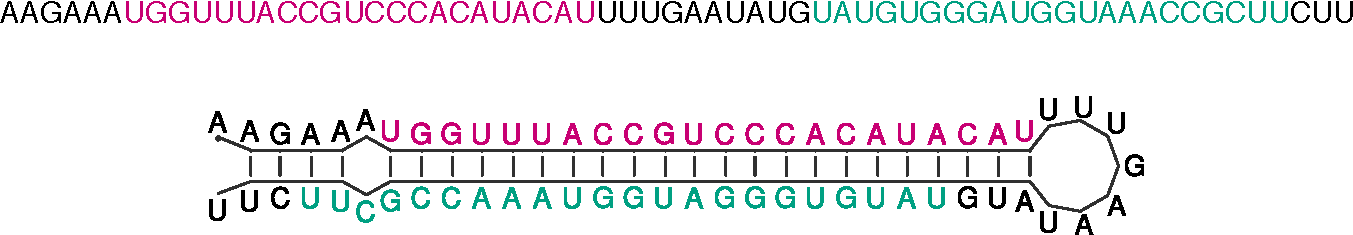
\includegraphics[width=.85\textwidth]{res/hsa-mir-299_ss.pdf}
  \caption{\small\slshape Secuencia
    (arriba) y estructura secundaria tipo horquilla (abajo) del
    pre-miRNA \textbf{hsa-mir-299}.  }
  \label{horquilla}
\end{figure}

El debate acerca del número e identidad de los miRNA presentes en
diferentes genomas es una cuestión abierta: a modo de ejemplo, para el
caso del genoma humano se había estimado inicialmente que se
encontrarían unos pocos cientos de genes miRNA; posteriormente este
número ha sido revisado a unos 1000 \cite{sewer}\cite{chang}.
Actualmente, se encuentra que el número de miRNA descubiertos en
humanos duplica esta cifra \cite{gomes}.  Teniendo en cuenta que estas
predicciones consideran sólo aquellos miRNA que se encuentran
conservados entre especies relativamente distantes (como primates y
roedores) y no aquellos de evolución más reciente \cite{sewer}, el
número de miRNA en humanos podría ser mucho mayor que las
estimaciones. La base de datos miRBase \cite{mirbase2}\cite{mirbase3}
recopila el conjunto de (pre-)miRNA conocidos hasta la
fecha. En la última versión disponible (r.19, agosto de 2012) se listan
21264 pre-miRNA experimentalmente validados, conteniendo un total de
25141 miRNA maduros, para 193 especies diferentes.
%

En principio, la identificación de nuevos pre-miRNA se realiza en forma
experimental en el laboratorio. Ésta es la primera elección, pero sólo
aquellos pre-miRNA abundantes pueden ser detectados de forma fiable
mediante esta técnica. Sin embargo, no todos los pre-miRNA están bien
expresados en múltiples tipos de tejidos: aquellos pre-miRNA que tienen un
bajo nivel de expresión, que se expresan en tejidos específicos y/o
que se presentan sólo en determinados estadíos de desarrollo celular
pueden ser fácilmente ignorados mediante la técnica
experimental \cite{ding}\cite{xu}.  En pos de superar estas
dificultades propias del método experimental es que surgen técnicas
computacionales para encontrar aquellos pre-miRNA que son específicos a
determinados tipos de tejidos o estadíos de desarrollo celular, y
aquellos escasamente expresados \cite{sheng}\cite{xu}.

Los métodos computacionales para el reconocimiento de genes pre-miRNA se
han desarrollado en dos direcciones principales: los métodos
comparativos, basados en la conservación ya sea de la secuencia y/o la
estructura secundaria entre distintas especies, y los no comparativos,
basados en el aprendizaje de máquina o Inteligencia
Computacional. Estos dos enfoques se complementan mutuamente al
encarar distintas estrategias para la predicción de nuevos pre-miRNA
\cite{batuwita}\cite{sheng}.

En un enfoque comparativo, se analizan genomas de diferentes especies
buscando correspondencias que cumplan con las características de un
pre-miRNA. Tal como en el caso del método experimental, mediante esta
técnica sólo es posible detectar aquellos pre-miRNA conservados entre
especies y con un elevado nivel de expresión. En cambio, en un enfoque
no comparativo se utiliza alguna técnica de aprendizaje de máquina,
para generar un modelo computacional que describe internamente las
características del pre-miRNA a partir de un conjunto de datos que se
utilizan en la etapa del entrenamiento. Con este modelo computacional
se genera un \emph{clasificador}.

El objetivo último de un clasificador no comparativo es obtener una
tasa mínima de errores de clasificación para conjuntos de datos
nuevos, que no hayan sido utilizados en la etapa de entrenamiento.  En
Inteligencia Computacional se pueden utilizar diversas técnicas para
la implementación de un clasificador no comparativo, entre ellas
el \emph{Perceptrón Multicapa}
\cite{mlp1}\cite{mlp2} y la \emph{Máquina de Vectores de Soporte}
\cite{svm}.  El Preceptrón Multicapa (\emph{MLP}, del inglés
\eng{Multilayer Perceptron}) es un tipo de red neuronal artificial con
propagación hacia adelante, donde las neuronas se disponen en capas.
La salida de cada neurona se determina al aplicar una \emph{función de
  activación}, de tipo sigmoidea, a la suma ponderada de las salidas
en la capa anterior. Durante el entrenamiento del MLP se ajustan los
pesos de cada neurona mediante un algoritmo de aprendizaje basado en
la \emph{retropropagación} del error de clasificación, hasta obtener
una tasa de clasificación satisfactoria \cite{jain}.  La Máquina de
Vectores de Soporte (\emph{SVM}, de su nombre en inglés \eng{Support
  Vector Machine}) es un algoritmo de clasificación que se basa en
transformar, mediante una función de transformación llamada \emph{núcleo}, el
espacio $N$-dimensional de los datos de entrada en otro espacio de
dimensión $M: M\gg N$, donde se espera que los datos sean linealmente
separables mediante un hiperplano. El entrenamiento consiste en
encontrar el hiperplano óptimo de separación para el conjunto de datos
presentado \cite{bottou}.

\section{Verificar lo que sigue}
En el Centro de Investigación en Señales, Sistemas e Inteligencia
Computacional \emph{sinc(i)} de la Facultad de Ingeniería y Ciencias
Hídricas surge la necesidad de contar con un clasificador de
pre-miRNA. Al revisar los desarrollos publicados en el tema, se
encuentra que en muchos de ellos las tasas de clasificación no son
satisfactorias, en otros casos, se obtienen buenas tasas de
clasificación sólo en casos particulares.  En muchos de estos trabajos
no se encuentra disponible el código fuente, lo que imposibilita su
implementación en forma directa.  Además, en aquellos casos en que sí
se publica el código fuente, se encuentra que tanto el lenguaje de
programación utilizado como el formato de entrada/salida varían entre
diferentes trabajos.  Teniendo en cuenta estos inconvenientes es que
se propone en este trabajo desarrollar un método informático para la
identificación de pre-miRNA mediante un clasificador de tipo
no comparativo, que haga uso de técnicas de Inteligencia Computacional
para el reconocimiento de patrones.  Tomando como base aquellos
métodos que se encuentran en la bibliografía, se generará un método
propio con el objetivo de lograr una tasa de clasificación máxima.

Para cada entrada presentada, el método deberá ser capaz de
discriminar entre dos \emph{clases}: positiva para aquellas que
corresponden a un pre-miRNA y negativa para aquellas entradas que no
lo son.  Una secuencia de pre-miRNA se representa mediante una cadena
de caracteres \mono{A, G, C, U,} donde cada carácter representa el
tipo de \emph{base} constitutiva de cada nucleótido\footnote{Las bases
  constitutivas del ARN son: \emph{adenina}, \emph{guanina},
  \emph{citosina} y \emph{uracilo}, de ahí la representación \mono{A,
    G, C, U}.}.  A partir de esta secuencia, mediante un proceso de
extracción de características se generará un vector numérico que será
la entrada al clasificador.  Para el clasificador se utilizará la
Máquina de Vector de Soporte (SVM), ya que se observa en la
bibliografía que esta técnica presenta un buen desempeño en esta clase
de problemas, junto con el Perceptrón Multicapa (MLP), técnica
relacionada a la SVM \cite{collobert} que se dicta en la materia
Inteligencia Computacional de la Carrera, con el propósito de estudiar
su desempeño en este tipo de problemas de clasificación.  La salida
del método será de tipo binaria, con formato a especificar, en donde
cada uno de los dos valores posibles se corresponderá con las clases
\emph{pre-miRNA} y \emph{no-pre-miRNA}.

Se seleccionarán conjuntos de datos tanto positivos como negativos
para el entrenamiento del clasificador. Como conjunto de datos
positivos, se deberán utilizar pre-miRNAs validados experimentalmente.
Para el caso negativo, se deberán utilizar datos artificialmente
seleccionados que no contengan pre-miRNAs, aunque sí presenten
características similares a éstos.

El impacto social del desarrollo de este proyecto se verá en un
aumento en la productividad de los investigadores del área al
posibilitarle una mayor facilidad de acceso que los sistemas actualmente
disponibles. También se pretende que sirva como puntapié inicial en
desarrollos futuros de sistemas similares con mayor complejidad y
rendimiento. En una visión englobadora, se agilizará la investigación
en el área con las implicancias que esto trae a la sociedad en
general, como el desarrollo de nuevos métodos de prevención y
tratamiento de enfermedades de diversa índole en las personas,
animales y plantas; y una mayor y mejor comprensión de los procesos
involucrados en su aparición y desarrollo.

El alumno considera que en lo personal, el desarrollo de este proyecto
le permitirá profundizar su conocimiento en diferentes áreas de la
Inteligencia Computacional, así como su aplicación al campo de la
bioinformática. Expresa que el desarrollo de este proyecto le
permitirá desarrollar habilidades y conocimientos que le serán de gran
valor en el desempeño como profesional, y en caso de seguir una
carrera de investigación servirá de introducción informal a la
metodología de trabajo en este campo.
%
%
%
\chapter{Estudios}
%
%
\section{Introducción}
En este informe entregable se presenta una revisión de las tareas
llevadas a cabo por el alumno tal como se ha estipulado en la
Propuesta de Proyecto Final de Carrera.

El documento se divide en las secciones: Bibliografía consultada,
Bases de datos recopiladas, Codificación de clasificadores de prueba
y Armado de la base de datos definitiva.

En pos de evitar la incorporación del código fuente generado en el
documento, se refiere al lector al repositorio disponible en
\url{https://github.com/maurete/pfc/}, donde se puede consultar
el código fuente y demás archivos generados durante el desarrollo.
%
%
%
%
\section{Bibliografía consultada}
\label{bibliografia}
%
A continuación se enumera la bibliografía consultada, referente a la
perspectiva biológica de los pre-miRNA, las técnicas de clasificación
SVM y MLP, y diferentes implementaciones de clasificadores pre-miRNA
utilizando estas técnicas de Inteligencia Computacional. Se presenta
una breve reseña orientativa junto a cada publicación.
%
\subsection{D. P. Bartel \cite{bartel116}}
Este trabajo brinda una revisión de los desarrollos en la
investigación de los microRNAs y las conclusiones que surgen de éstos
acerca de la biogénesis y función de los miRNAs.  Ofrece una
explicación didáctica del proceso de maduración de un pre-miRNA en
miRNA.  Publicado en 2004, es anterior a la aparición de los métodos
computacionales no-comparativos que permitieron un gran aumento en el
número de nuevos miRNAs descubiertos.
%
\subsection{L. Li et al. \cite{lili}}
En este trabajo, publicado en 2010, se ofrece un panorama de diversos
métodos para la identificación de miRNAs junto a una revisión de las
características biológicas de los mismos. Se presentan métodos tanto
de tipo comparativo como aquellos basados en aprendizaje de máquina,
así como métodos que trabajan sobre los datos experimentales de
técnicas de secuenciamiento en gran escala o \eng{deep sequencing}.
También se presenta el estado del arte en la predicción de dianas
(\eng{targets}) y regulación de la expresión de los miRNAs.
%
\subsection{D. Yue et al. \cite{yue}}
Se presenta en este trabajo un resumen de las técnicas disponibles
para la predicción de dianas y de métodos de predicción de las
funciones de los miRNAs, con una exposición clara de los conceptos
relevantes en este campo de estudio.
%
\subsection{L. Bottou y C.-J. Lin \cite{bottou}}
Este trabajo presenta una descripción del problema general de
clasificación mediante SVM \cite{svm}, detallando el problema de
optimización a resolver y los parámetros a considerar en la
utilización e implementación de las máquinas de vectores de soporte.
%
\subsection{C. Xue et al. \cite{xue}}
%
En este trabajo se presenta un clasificador de secuencias de
pre-microRNA mediante SVM \cite{svm}.  En el clasificador se utiliza
un conjunto de características de tipo estructura-secuencia,
utilizando como entrada al clasificador un vector de frecuencia de 32
``triplets'' que combinan el nucleótido de la secuencia con la
estructura secundaria del entorno donde éste se presenta.

El método aquí descripto es notable en que obtiene una buena tasa de
clasificación utilizando una combinación simple de características de
la secuencia y la estructura secundaria.
%
\subsection{S. K. L. Ng y S. K. Mishra \cite{ng}}
%
En este trabajo se presenta un clasificador de secuencias de
pre-miRNA mediante SVM.

El conjunto de características utilizado consiste en 29 medidas
``globales e intrínsecas'' a la secuencia y su estructura secundaria:
(1) 17 medidas de composición de la secuencia: frecuencia de
ocurrencia de dinucleótidos
$\mono{XY}:(\mono{X},\mono{Y})\in\{\mono{A},\mono{G},\mono{C},\mono{U}\}$
y frecuencia agregada de ocurrencia de los nucleótidos \mono{G} y
\mono{C}; (2) 6 medidas de plegado basadas en la mínima energía libre
y la distribución de los pares de bases; (3) un descriptor
topológico; y (4) 5 variantes normalizadas de estas características.

El método además es probado para detectar pre-miRNAs en genes de
virus, recorriendo éste mediante una ventana deslizante de 95nt y
clasificando las secuencias extraídas.
%
\subsection{R. Batuwita y V. Palade \cite{batuwita}}
En esta publicación se describe un método de clasificación de
pre-miRNAs que elabora sobre \cite{ng} incorporando características
basadas en la mínima energía libre, otras características relacionadas
el programa RNAfold, y características basadas en los pares de bases.

Se discute acerca de la relevancia de cada una de las características
y se presenta luego un conjunto reducido de éstas para mejorar la
performance del clasificador, y también se discute acerca del problema
de \emph{desbalance de clases}, siempre presente en la
clasificación de pre-miRNAs.
%
\subsection{S. Sewer et al. \cite{sewer}}
Este trabajo describe un método de predicción de microRNAs en el
genoma homano, de rata y de ratón. El método tiene un enfoque
comparativo para la selección de las regiones candidatas del genoma,
así como un enfoque no-comparativo para la predicción de los microRNAs
en estas regiones. Para la clasificación se utilizan Máquinas de
Vector de Soporte.
%
\subsection{J. Hertel y P. F. Stadler \cite{hertel}}
Este trabajo presenta un método de clasificación de pre-miRNAs basado
en características de la secuencia y de la estructura secundaria, con
un clasificador basado en SVM. Como paso inicial se utiliza una
técnica de ``alineación múltiple'' de la secuencia, ajustando una
ventana para determinar la posición exacta del pre-miRNA candidato en
la región.  El resultado es una elevada especificidad del 99\% (muy
pocos falsos positivos), con una sensibilidad del 80\%.
%
\subsection{Y. Xu et al. \cite{xu}}
En este trabajo se presenta un método no-comparativo que en lugar de
utilizar un método de aprendizaje supervisado como SVM, utiliza un
algoritmo de \eng{ranking} basado en \eng{random walks}.  Este método
se caracteriza por no requerir de ejemplos negativos para el
entrenamiento. Finalmente el método es aplicado para la identificación
de nuevos pre-miRNAs en \eng{Anopheles gambiae}, un mosquito que es el
principal vector de la malaria en África.
%
\subsection{J. Ding et al. \cite{ding}}
Este trabajo presenta un método de clasificación mediante SVM con un
enfoque específicamente diseñado para resolver el problema de
desbalance de ejemplos positivos y negativos, y que a la vez no asume
características estructurales de los pre-miRNAs.

Se describe la utilización conjunta de diferentes clasificadores SVM
para reducir los problemas del desbalance de clases. Por otro lado
incorpora características de pre-miRNAs tipo multi-loop y realiza una
selección del conjunto de características finales a considerar
mediante la técnica \eng{F-score}, que permite seleccionar aquellas
características de entrada más ``relevantes'' para el clasificador.
%
%
%
%
\section{Bases de datos recopiladas}
%
Tomando como base los métodos de clasificación de pre-miRNAs
consultados en la bibliografía se procedió a revisar los respectivos
materiales suplementarios en búsqueda de bases de datos completas
sobre las cuales trabajar.  A continuación se describen las bases de
datos recopiladas a partir de los materiales suplementarios de
\cite{xue}, \cite{ng} y \cite{batuwita}.
%
\subsection{Triplet-SVM \cite{xue}}
%
Si bien en la página del
autor\footnote{\url{http://bioinfo.au.tsinghua.edu.cn/software/mirnasvm/}}
ya no están disponibles los datos, éstos se pueden encontrar en una
versión anterior de la misma, disponible en el archivo de
internet\footnote{\url{http://web.archive.org/web/20120210235054/http://bioinfo.au.tsinghua.edu.cn/software/mirnasvm/}}.
%
\subsubsection{Características disponibles}
En esta base de datos cada una de las entradas presenta las siguientes
características:
\begin{description}
  [style=sameline,leftmargin=3cm,itemsep=6pt]
%
\item[identificador] cadena de caracteres, p. ej. \mono{hsa-mir-100}.
%
\item[secuencia] cadena de caracteres \mono{A}, \mono{G}, \mono{C},
  \mono{U}.
%
\item[estructura secundaria] cadena de caracteres \mono{(}, \mono{.},
  \mono{)}. Calculada con el programa RNAfold \cite{vienna}.
%
\item[SEQ\_LENGTH] longitud de la secuencia considerada para el armado
  del vector de características. Cuenta aquellos nucleótidos que
  pertenecen al tallo del pre-miRNA.
%
\item[GC\_CONTENT] se define según
  $\frac{\T{cant}(\mono{G})+\T{cant}(\mono{C})}{\mono{SEQ\_LENGTH}}$,
  donde $\T{cant}(x)$ cuenta el número de ocurrencias del nucleótido
  $x$ en el tallo del pre-miRNA.
%
\item[BASEPAIR] cantidad de nucleótidos
  que forman un par de bases en el pre-miRNA.
%
\item[FREE\_ENERGY] mínima energía libre de plegado
  obtenida con RNAfold.
%
\item[LEN\_BP\_RATIO] se define según
  $\frac{\mono{SEQ\_LENGTH}}{\mono{BASEPAIR}}$.
\end{description}
%
El vector de 32 triplets utilizados en el clasificador no está
directamente disponible, si bien se pueden encontrar las rutinas para su
cálculo, en lenguaje Perl.
%
\subsubsection{Conjuntos de datos}
\paragraph{pre-miRNAs humanos}
\begin{description}[style=nextline,leftmargin=5cm,align=right]
\item[Tipo:] Conjunto de entrenamiento (163) y prueba (30), datos
  positivos
\item[Núm. entradas:] 193
\item[Especies:] Homo sapiens (hsa)
\item[Descripción:] Tomados de miRNA registry rel 5.0, sept/2004
\end{description}
\paragraph{CROSS-SPECIES}
\begin{description}[style=nextline,leftmargin=5cm,align=right]
\item[Tipo:] Conjunto de prueba, datos positivos
\item[Núm. entradas:] 581
\item[Especies:] mmu (36), rno (25), gga (13), dre (6), cbr (73), cel
  (110), dps (71), dme (71), osa (96), ath (75), ebv (5)
\item[Descripción:] Tomados de miRNA registry rel 5.0, sept/2004
\end{description}
%
\paragraph{pre-miRNAs humanos (actualizado)}
\begin{description}[style=nextline,leftmargin=5cm,align=right]
\item[Tipo:] Conjunto de prueba, datos positivos
\item[Núm. entradas:] 39
\item[Especies:]  Homo sapiens (hsa)
\item[Descripción:] Conjunto de 39 pre-miRNAs obtenido a partir de los
  89 reportados en \cite{bentwich}, eliminando entradas redundantes y
  aquellas similares a las encontradas en el conjunto de
  entrenamiento.
\end{description}
%
\paragraph{CONSERVED-HAIRPIN}
\begin{description}[style=nextline,leftmargin=5cm,align=right]
\item[Tipo:] Conjunto de prueba, datos mayormente negativos (algunos
  positivos)
\item[Núm. entradas:] 2444
\item[Especies:]  Homo sapiens (hsa)
\item[Descripción:] Se obtiene mediante aplicación de una ventana
  deslizante de 100nt con paso 10nt en la región 56000001--57000000
  del cromosoma humano 19 de UCSC database. La gran mayoría de
  entradas en este conjunto son pseudo-pre-miRNAs, aunque contiene
  algunos pre-miRNAs reales.  Por esto se deberá usar únicamente como
  conjunto de prueba.
\end{description}
%
%
%
%% \begin{tabular}{@{}p{2.8cm}p{1.2cm}p{1.6cm}p{8.6cm}@{}}
%% \toprule
%% Tipo & Elems. & Especies & Descripción \\ \midrule
%% \mcol{4}{l}{CODING} \\ \midrule[.2pt]
%% Entrenamiento, datos negativos &
%% 8494 &
%% Homo sapiens (hsa) &
%%  Entradas obtenidas de las regiones codificantes
%%   (CDS) de los genes humanos RefSeq disponibles en en la base de datos
%%   USC.  Para el armado de este conjunto se consideran los siguientes
%%   criterios:
%%   \begin{itemize}
%%   \item Mínimo de 18 pares de bases en el tallo
%%   \item Máximo -15kcal/mol de energía libre mínima
%%   \item Ningún bucle múltiple (no más de un ``tallo'' en la estructura
%%     secundaria)
%%   \end{itemize}
%% \\ \bottomrule
%% \end{tabular}
%
%
%
%
%
\newpage
\subsection{miPred \cite{ng}}
Los conjuntos de datos de este trabajo están disponibles en la página
del autor\footnote{\url{http://web.bii.a-star.edu.sg/archive/stanley/%
Publications/Supp_materials/06-002-supp.html}}.
%
\subsubsection{Características disponibles}
\begin{description}%
  [style=sameline,leftmargin=5cm,itemsep=4pt]
%
\item[identificador] cadena de caracteres, p. ej. \mono{hsa-let-7a}.
%
\item[secuencia] cadena de caracteres \mono{A}, \mono{G}, \mono{C},
  \mono{U}.
%
\item[estructura secundaria] cadena de caracteres \mono{(}, \mono{.},
  \mono{)}.
%
\item[longitud] de la secuencia completa.
%
\item[A, G, C, U] (x4) número de ocurrencias del nucleótido en la
  secuencia.
%
\item[G+C, A+U] (x2) suma de las ocurrencias de \mono{G} y \mono{C}, y
  \mono{A} y \mono{U} respectivamente.
%
\item[AA, AG, AC, \textellipsis, UU] (x16) número de ocurrencias del
  dinucleótido correspondiente en la secuencia.
%
\item[\%A, \%G, \%C, \%U] (x4) frecuencia de ocurrencia del nucleótido
  correspondiente.
%
\item[\%(G+C), \%(A+U)] (x2) frecuencia de ocurrencia de
  \mono{G}+\mono{C} y \mono{A}+\mono{U}.
%
\item[\%AA, \%AG, \%AC, \textellipsis] (x16) frecuencia de ocurrencia
  de los dinucleótidos correspondientes.
%
\item[pb] cantidad de pares de bases.
%
\item[mfe] mínima energía libre según RNAfold.
%
\item[Q] \emph{entropía de Shannon}\footnote{La entropía de Shannon
  es una medida de aleatoriedad utilizada en Teoría de la
  Información. En forma simple, podemos decir que muestra en cuánto se
  diferencia una secuencia determinada de otra completamente
  aleatoria, y de esta manera brinda una idea de la cantidad de
  información contenida en la misma.} de la secuencia.
%
\item[D] distancia entre pares de bases.
%
\item[Npb, Nmfe, NQ, ND] (x4) valores normalizados de \mono{pb},
  \mono{mfe}, \mono{Q}, \mono{D} por la longitud de la secuencia.
%
\end{description}
%
%
\subsubsection{Conjuntos de datos}
\paragraph{pre-miRNAs no redundantes}
\begin{description}[style=nextline,leftmargin=5cm,align=right]
\item[Tipo:] Conjunto de datos positivos
\item[Núm. entradas:] 2241
\item[Especies:] 45 especies agrupadas en artropoda, nematoda,
  vertebrata, viridiplantae y virus
\item[Descripción:] Tomados de miRBase 8.2 (jul/2006) para todas las
  especies disponibles, se filtran aquellas secuencias redundantes
  mediante un algoritmo de agrupación incremental
  ``ávido''\cite{greedy}.
\end{description}

\paragraph{ncRNAs funcionales}
\begin{description}[style=nextline,leftmargin=5cm,align=right]
\item[Tipo:] Conjunto de datos negativos
\item[Núm. entradas:] 12387
\item[Especies:] muchas (prokaryota y eukaryota)
\item[Descripción:] Tomados de Rfam 7.0, consiste en un conjunto de
  ncRNAs de los que se han eliminado 46 tipos de pre-miRNAs.
\end{description}

\paragraph{mRNAs}
\begin{description}[style=nextline,leftmargin=5cm,align=right]
\item[Tipo:] Conjunto de datos negativos
\item[Núm. entradas:] 31
\item[Especies:] varias, entre ellas: perro, hsa, mmu, cel, rno,
  \textellipsis.
\item[Descripción:] Consiste en 31 mRNAs mensajeros que se pliegan en
  estructuras complejas con MFEs extremadamente negativas. Tomados de
  GeneBank DNA Database.
\end{description}

\paragraph{pseudo-hairpins}
\begin{description}[style=nextline,leftmargin=5cm,align=right]
\item[Tipo:] Conjunto de datos negativos
\item[Núm. entradas:] 8494
\item[Especies:] homo sapiens (hsa)
\item[Descripción:] Ídem al dataset CODING de triplet-svm, en este
  caso con más características extraídas.
\end{description}
%
%
%
%
%
\subsection{microPred \cite{batuwita}}
En esta base de datos están presentes las características presentadas
en \cite{ng} (salvo estructura secundaria) y se introducen otras 19 
características adicionales. De estas 19 se detallan sólo aquellas que están
basadas en la secuencia y/o estructura secundaria, el resto de características
se basa en descriptores moleculares, y dada su complejidad de cálculo
se consideran fuera del alcance del actual proyecto.
%
Los datos se encuentran disponibles en el sitio web de los autores%
\footnote{\url{http://www.cs.ox.ac.uk/people/manohara.rukshan.batuwita/microPred.htm}}.
%
\newpage
\subsubsection{Características disponibles}
\begin{description}
  [style=sameline,leftmargin=5cm,itemsep=4pt]
%
\item[identificador] cadena de caracteres, p. ej. \mono{hsa-let-7a}.
%
\item[secuencia] cadena de caracteres \mono{A}, \mono{G}, \mono{C},
  \mono{U}.
%
\item[MFEI$_3$] \mono{Nmfe} dividida entre el número de loops (bucles)
  de la estructura secundaria.
%
\item[MFEI$_4$] \mono{mfe} dividida entre el número de pares de bases.
%
\item[|A-U|/L, |G-C|/L, |G-U|/L] (x3) número de pares de bases
  \mono{A-U}, \mono{G-C} y \mono{G-U} respectivamente, normalizados
  por la longitud de la secuencia.
%
\item[Avg\_BP\_Stem] número de pares de bases dividido entre el
  número total de tallos en la estructura secundaria.
%
\item[\%(A-U)/n\_stems, \%(G-C)/n\_stems, \%(G-U)/n\_stems] (x3) con
  \mono{\%(X-Y)} la frecuencia del par de bases \mono{X-Y}, dividido
  por el número de tallos en la estructura secundaria.
\end{description}
%
%
\subsubsection{Conjuntos de datos}
\paragraph{pre-miRNAs humanos}
\begin{description}[style=nextline,leftmargin=5cm,align=right]
\item[Tipo:] Conjunto de datos positivos
\item[Núm. entradas:] 691
\item[Especies:] Homo sapiens (hsa)
\item[Descripción:]Tomados de miRBase 12. Contiene 660 pre-miRNAs
  single-loop y 31 multi-loop.
\end{description}
%
\paragraph{pseudo-hairpins}
\begin{description}[style=nextline,leftmargin=5cm,align=right]
\item[Tipo:] Conjunto de datos negativos
\item[Núm. entradas:] 8494
\item[Especies:] Homo sapiens (hsa)
\item[Descripción:] Ídem dataset CODING de Xue, con más
  características extraídas.
\end{description}
%
\paragraph{Otros ncRNAs humanos}
\begin{description}[style=nextline,leftmargin=5cm,align=right]
\item[Tipo:] Conjunto de datos negativos
\item[Núm. entradas:] 754
\item[Especies:] Homo sapiens (hsa)
\item[Descripción:] Conjunto de datos compilado manualmente por los
  autores. Contiene ncRNAs humanos que no son pre-miRNAs.
\end{description}
%
%
%
%
\section{Codificación de clasificadores de prueba}
\label{pruebas}
%
Una vez obtenidas las bases de datos se procedió a codificar
algoritmos de clasificación preliminares.
Se optó por trabajar con el conjunto de datos de \cite{xue},
intentando replicar los resultados obtenidos en ese trabajo mediante
la utilización de herramientas propias. Según se ha observado en la
bibliografía, este trabajo es tomado como modelo de referencia debido a
la simplicidad del método y los buenos resultados que obtiene.

Al analizar el formato de los datos disponibles surge la necesidad
de codificar una herramienta para el manejo de archivos en formato
FASTA\footnote{FASTA es un formato de texto para la representación
  de secuencias de nucleótidos, como es el RNA.
  La especificación se encuentra disponible en
  \url{http://blast.ncbi.nlm.nih.gov/blastcgihelp.shtml}.}.
El formato de salida del programa \mono{RNAFold} es además
muy similar a FASTA, e incorpora la información de la estructura
secuendaria o \emph{plegado} para cada entrada.
%
Se ha codificado la herramienta \mono{fautil.py} en lenguaje Python,
que permite manipular archivos con formato FASTA/RNAfold. También para
Matlab se ha codificado la utilidad \mono{fastaread.m} para lectura
de estos archivos.
%
\subsection{Extracción de características}
%
Tal como en \cite{xue}, se definen 32 elementos ``triplete'', que
relacionan en cada posición la secuencia con la estructura secundaria
en el entorno. Para cada entrada de la base de datos, se calcula la
frecuencia de ocurrencia de cada triplete, generando así un 32-vector
que se utiliza como entrada al clasificador.

%% Tal como en \cite{xue}, se define un ``triplete'' las características
%% se calculan para cada ``triplete'' (\emph{triplet}) en la secuencia,
%% relacionando secuencia y estructura secundaria. Para cada entrada, el
%% vector de características representa la frecuencia de ocurrencia de
%% las 32 configuraciones posibles al combinar el nucleótido central del
%% triplete con la estructura secundaria del mismo.

El proceso detallado se puede describir como sigue:
\begin{enumerate}
\item A partir de la estructura secundaria, se determina una región a
  considerar para los cálculos, de forma que excluya los extremos
  ``sueltos'' así como el bucle central de la cadena, donde las bases
  no forman pares.
\item Se recorre en esta región tanto la secuencia como la
  estructura secundaria con una ventana de 3nt y paso 1nt. En cada
  paso:
  \begin{enumerate}
  \item Se calcula una cadena de ``elemento triplet'' añadiendo al
    caracter central en la secuencia los tres caracteres
    correspondientes a la estructura secundaria (se ignora la
    orientación en el caso de bases que forman un par). Se obtiene
    así, por ejemplo, el elemento ``\mono{A.((}''.
  \item Se incrementa el contador de ocurrencias para el elemento en
    la posición correspondiente del vector.
  \item En los extremos se ignora un caracter del triplet, que se
    considera en la estructura secundaria como un ``\mono{.}''.
  \end{enumerate}
\item Se normaliza el vector de frecuencias dividiéndolo por el número
  total de triplets contados.
\end{enumerate}

En el archivo \mono{fautil.py}, rutina \mono{triplet}, se encuentra
una implementación en Python de este proceso. También se ha codificado
el mismo algoritmo en Matlab, \mono{triplet.m}.
%
\subsection{Clasificadores}
Se generaron 3 clasificadores, según se detallan a continuación.
\begin{enumerate}
\item Clasificador mediante SVM utilizando \emph{libsvm}\cite{libsvm} con los
  parámetros por defecto.
\item Clasificador mediante SVM utilizando el \emph{Bioinformatics
  Toolbox} de Matlab.
\item Clasificador mediante MLP utilizando el \emph{Neural Network
  Toolbox} de Matlab.
\end{enumerate}
%
La librería \emph{libsvm}\cite{libsvm} provee una utilidad \mono{svm-easy} que
busca en forma automática aquellos parámetros que minimizan el
error. En los otros casos, esta búsqueda se realizó en forma manual,
ajustando los parámetros \mono{boxconstraint} y y \mono{sigma} para
SVM y para MLP ajustando el número de capas ocultas y el número de
nodos por capa oculta.
%
\subsection{Pruebas}
Los clasificadores se entrenaron con el mismo conjunto de datos de
\cite{xue}, y se probaron con los conjuntos de prueba \emph{Real} (30
elementos), \emph{Pseudo} (1000 elementos) y \emph{Updated} (39
elementos), también de la misma fuente.

En el caso de SVM-Matlab y MLP, se probaron diversos parámetros hasta
encontrar aquellos que obtienen el mejor rendimiento del clasificador.
En la tabla \ref{testresults} se presentan figuras de rendimiento para
los distintos clasificadores. %En el caso de SVM-Matlab se muestran
%tres resultados representativos correspondientes a diferentes
%parámetros. 
En el caso MLP, se encontró que los resultados no varían
significativamente para distintas configuraciones, con diferencias
menores a 3\% en cada caso.  Se muestran entonces para MLP tasas
representativas.
%
\begin{table}
  \caption{Resultados de las pruebas iniciales de clasificación}
  \center%\sffamily
  \begin{tabular}{lrrr}\toprule
    Clasificador  & \% Real (/30) &
                     \% Pseudo (/1000) & \% Updated (/39) \\\midrule
    Triplet-SVM   &  $93.3$    & $88.1$     & $92.3$     \\
    SVM (libSVM)  & $100.0$    & $87.4$     & $92.3$     \\
    SVM (Matlab)  & $100.0$    & $91.2$     & $89.7$     \\
    %% svm (matlab,2) & $96.7$     & $96.6$     & $48.7$     \\
    %% svm (matlab,3) & $100.0$    & $86.4$     & $97.4$     \\
    MLP           &  $90.0$    & $85.0$     & $91.0$  \\\bottomrule
  \end{tabular}
  \label{testresults}
\end{table}
%

Como se puede observar en la tabla \ref{testresults}, las tasas de
clasificación para los distintos conjuntos resultan satisfactorias, e
incluso sensiblemente mejores a aquellas del trabajo original.  Sin
embargo, estos números deberán tomarse con cuidado, ya que han sido
obtenidos entrenando y validando con particiones estáticas, y podrían
ser resultado de un sobreentrenamiento para estos datos en
particular. Se observa también que el perceptrón multicapa presenta
una buena tasa de clasificación incluso cuando se trata de una única
neurona (sin capas ocultas), siempre para este mismo conjunto de
datos.

Se ha implementado el script \mono{triplet\_libsvm.sh} para las
pruebas con \emph{libsvm}, y los scripts \mono{triplet\_svm.m} y
\mono{triplet\_mlp.m} para las pruebas en Matlab de los clasificadores
SVM y MLP respectivamente. Con el software apropiado, estos scripts
se pueden ejecutar directamente para reproducir los resultados de las
pruebas.
%
%
%

\chapter{Estudios/Análisis}
%
%
\section{Armado de la base de datos definitiva}
Para el armado de la base de datos definitiva se tomaron como fuente
los conjuntos de datos y características utilizados en \cite{xue},
\cite{ng} y \cite{batuwita}. Se incorporó al conjunto de datos
la última versión disponible de miRBase \cite{mirbase2}.

Como primer paso se procedió a validar el plegado de las secuencias en
las bases de datos originales aplicando el programa RNAfold sobre las
mismas y comprobando que el plegado obtenido fuera el mismo que el
presente en la base de datos original. Se utilizó la versión 1.8.5 de
RNAfold, ya que con la versión actual (2.1) se obtienen plegados
diferentes en la mayoría de los casos.

Una vez validadas las estructuras secundarias se procedió a filtrar
aquellas entradas con bucles múltiples en la estructura secundaria, ya
que las características de triplete no están definidas en estos casos.
De esta manera se eliminó la base de datos ``mRNA'' de \cite{ng} por
completo, ya que todas las entradas en este caso poseen bucles
múltiples.

Luego se procedió a la ectracción y validación de características
extraídas contra las bases de datos respectivas: las características
de triplete y triplete-extra contra la base de datos de \cite{xue},
las características de la secuencia contra la base de \cite{ng}, y las
de estructura secundaria con la base de datos en \cite{batuwita}.

Además de las características calculadas, se incorporan a la base de
datos los datos de la secuencia y estructura secundaria en formato
compatible RNAfold, junto con otro archivo donde se indica la clase
(pre-miRNA real, pseudo-pre-miRNA o indefinido) de cada entrada
correspondiente.  En el archivo \mono{README.md} de la base de datos
se detalla la estructura de directorios generada junto con el formato
de los archivos para cada caso.

Se codificó la herramienta \mono{feats.py} a partir de la utilidad
\mono{fautil.py}, para la extracción de características de archivos
con formato RNAfold. Se ignoraron aquellas características que no se
pueden calcular directamente con la información de la secuencia y de
la estructura secundaria.

Se codificó la herramienta \mono{tests.py} para la validación, así
como los scripts en Bash \mono{validate.sh} y \mono{generate\_db.sh},
los que pueden ser ejecutados directamente, siempre con el software
requerido, para validar y regenerar la misma base de datos a partir de
las fuentes.
%
\subsection{Características extraídas}
%
A continuación se enumeran las características disponibles en la base
de datos definitiva.
%
\subsubsection{Características de tripletes}
Vector de 32 elementos de tripletes, calculado según \cite{xue}.
Considerando la región del tallo, contiene el número de ocurrencias
del elemento triplete correspondiente, normalizado entre el número
total de ocurrencias.  El orden es el siguiente: \mono{A..., A..(,
  A.(., A.((, A(.., A(.(, A((., A(((, G..., G..(, G.(., G.((, G(..,
  G(.(, G((., G(((, C..., C..(, C.(., C.((, C(.., C(.(, C((., C(((,
  U..., U..(, U.(., U.((, U(.., U(.(, U((., U(((}.
%
\subsubsection{Características de tripletes ``extra''}
Características auxiliares que se obtienen
al calcular el vector de tripletes.
\begin{description}[style=sameline,leftmargin=5cm]
\item[length3] longitud de la secuencia considerada al
  extraer los elementos de triplete (número de bases que
  conforman el tallo de la estructura de horquilla).
\item[basepairs] número de pares de bases en
  el pre-miRNA.
\item[{length3/basepairs}] grado de complementariedad
  entre los dos brazos de la estructura de horquilla. Para una
  complementariedad perfecta se da el valor mínimo de 2, aumentando cuanto más
  bases ``sueltas'' contenga el tallo.
\item[gc\_content] $=(\T{cant(\mono{G})}+\T{cant(\mono{C})})/\mono{length3}$. Proporción de nucleótidos \mono{G} y
  \mono{C} en el tallo.
\end{description}
%
\subsubsection{Medidas de la secuencia}
%Este grupo contiene las siguientes medidas de la secuencia del pre-miRNA:
\begin{description}[style=sameline,leftmargin=5cm]
\item[length] longitud del pre-miRNA, incluyendo extremos sueltos y el
  bucle central.
\item[A, C, G, U] (x4) número de nucleótidos \mono{A}, \mono{C},
  \mono{G} y \mono{U}, respectivamente.
\item[G+C, A+U] (x2) número de nucleótidos \mono{G} y \mono{C}, y
  \mono{A} y \mono{U} respectivamente.
\item[XY] (x16) número de dinucleótidos (dos nucleótidos contiguos)
  \mono{XY}, con $\mono{X,Y}\in\{\mono{A,C,G,U}\}$. El orden es el
  siguiente: \mono{AC, AG, AU, CA, CC, CG, CU, GA, GC, GG, GU, UA, UC,
    UG, UU}.
\end{description}
%
\subsubsection{Medidas de la estructura secundaria}
%En este grupo se presentan las siguientes características relativas al
%plegado del pre-miRNA en su estructura de horquilla:
\begin{description}[style=sameline,leftmargin=5cm]
\item[MFE] Mínima Energía Libre obtenida al plegar la secuencia con
  \mono{RNAfold}.
\item[MFEI1] $={\mono{MFE}}/{(\mono{G+C})\cdot 100}$, con \mono{G+C}
  de las medidas de secuencia.
\item[MFEI4] $=\mono{MFE}/\mono{basepairs}$ con \mono{basepairs} de
  las características de triplete extra.
\item[dP] \mono{basepairs} normalizada con la longitud total
  \mono{length}.
\item[|A-U|/length] número de pares \mono{A-U} normalizado.
\item[|G-C|/length] número de pares \mono{G-C} normalizado.
\item[|G-U|/length] número de pares \mono{G-U} normalizado.
\end{description}
%
\subsection{Conjuntos de datos}
A continuación se listan los conjuntos de datos obtenidos en el armado
de la base de datos.
\begin{description}
\item[mirbase50] de \cite{xue}, contiene 1210 pre-miRNAs reales para
  diferentes especies, entre ellas 193 humanos, 112 de gallina, 207 de
  ratón, 172 de rata y 96 de arroz.
\item[updated] de \cite{xue}, contiene 39 pre-miRNAs humanos.
\item[coding] de \cite{xue}, contiene 8494 pseudo pre-miRNAs humanos.
\item[conserved-hairpin] de \cite{xue}, contiene 2444 pseudo
  pre-miRNAs humanos, aunque se conoce que algunos de ellos son
  pre-miRNAs reales. Se establece la clase para estas entradas como
  indeterminada, representada por el valor ambiguo 0.
\item[mirbase82-nr] de \cite{ng}, contiene 1985 pre-miRNAs de miRBase
  8.2 filtrados a 90\% de similaridad, para 40 especies incluyendo
  vertebrados, plantas y virus.
\item[functional-ncrna] de \cite{ng}, contiene 2657 ncRNAs
  funcionales, excepto pre-miRNAs, para varias
  especies.\item[mirbase12] de \cite{batuwita}, contiene 660
  pre-miRNAs humanos no redundantes originalmente de miRBase 12.0.
\item[other-ncrna] de \cite{batuwita}, contiene 129 ncRNAs humanos que
  no son pre-miRNAs.
\item[mirbase20] de \cite{mirbase2}, incorpora 21433 pre-miRNAs reales
  que no tienen bucles múltiples de miRBase 20, para 204 especies,
  entre ellos 1801 humanos, 1121 de ratón, 423 de rata y 392 de arroz.
\end{description}
%
%
%
\chapter{Análisis/Proyecto}
%
%
%
\section*{Introducción}
En el presente informe de avance se detalla el proceso de obtención de
un sistema de reconocimiento completo, desde la selección de los
clasificadores y su parametrización hasta la generación de la interfaz
de usuario de línea de comandos.

En la primera sección se presenta una introducción teórica de los
clasificadores, sus correspondientes parámetros de entrenamiento y los
métodos de selección de estos parámetros. En las secciones 2 y 3 se
describe la implementación y las pruebas realizadas para evaluación de
los métodos codificados. En la cuarta sección se especifica la
implementación del método definitivo y se presentan los resultados de
las pruebas finales de validación del método.
%
%
\section{Clasificadores}
%
El objetivo de un clasificador es asignar una clase a un patrón de
entrada. En el presente caso, se trata de determinar si un patrón dado
se corresponde o no con el de un pre-microRNA.

En el ámbito de la Inteligencia Computacional, un clasificador
consiste en un \emph{modelo}, que se obtiene a partir de un proceso de
entrenamiento en que se presentan al clasificador patrones de entrada
con su correspondiente clase. En términos generales, la generación del
modelo requiere de la especificación de \emph{parámetros} propios del
algoritmo de entrenamiento, además de los patrones del conjunto de
entrenamiento y sus etiquetas. De este modo se obtiene un método de
clasificación que posee \emph{capacidad de generalización} a partir de
la representación interna del modelo obtenida durante el
entrenamiento, y puede clasificar incluso patrones que no le han sido
presentados en dicho proceso.

Los patrones de entrada al clasificador son vectores numéricos de
longitud fija que se obtienen mediante el proceso de extracción de
características de los datos de entrada originales. Este proceso ha
sido especificado en el Informe de Avance anteriormente presentado.
%
%
\subsection{Perceptrón multicapa}
%
El perceptrón multicapa (MLP, \eng{Multilayer Perceptron})
\cite{mlp1,mlp2} es una red neuronal con propagación hacia adelante
(\eng{feedforward}), donde las neuronas se disponen en capas. La
primer capa, llamada de entrada, consiste en un conjunto de nodos
``sensores'' cuyas salidas corresponden al valor de cada componente
del vector de entrada. En las capas subsiguientes, llamadas
{ocultas}, se disponen de una serie de \emph{neuronas} (nodos
computadores).  La salida de cada neurona se determina al aplicar una
función de activación, de tipo sigmoidea, a la suma ponderada de las
salidas en la capa anterior.  Para el caso de un clasificador binario
tal como el considerado en el presente trabajo, la capa \emph{de
  salida} consiste en una única neurona, y el signo de su valor de
salida determina a qué clase corresponde el vector de entrada.

Dado el conjunto de entrenamiento $(\B{x}_i, y_i), i=1\ldots l$, con
una topología de la red fijada, el proceso de entrenamiento de un
clasificador MLP sigue, a grandes rasgos, los siguientes pasos:
\begin{enumerate}
\item Inicializar los pesos iniciales (ponderación) de cada neurona de
  forma aleatoria
\item Entrenar una \emph{época}:
  \begin{enumerate}
  \item Seleccionar el primer patrón y propagar hacia adelante: calcular
    la salida de cada neurona sucesivamente en cada capa hasta obtener
    la salida en la última capa.
  \item Ajustar los pesos de las neuronas mediante \emph{propagación hacia
    atrás}, basada en el gradiente de una función de error entre la salida
    obtenida y el valor esperado (la clase del patrón).
  \item Repetir a) y b) para todos los patrones de entrenamiento.
  \end{enumerate}
  \item Repetir 2 hasta satisfacer un criterio de corte.
\end{enumerate}
De este modo, se obtiene el modelo consistente en la red especificada
junto con los pesos obtenidos luego de haber entrenado con todo el
conjunto de entrenamiento. Los parámetros necesarios para la
generación de este modelo son entonces: el número de capas ocultas y
el número de neuronas en cada capa (la topología de la red), los
parámetros de la función de propagación hacia atrás tales como
la velocidad de aprendizaje, y el criterio de corte para
el entrenamiento, entre otros.
%
%
\subsection{Máquina de vectores de soporte}
%
La máquina de vectores de soporte (SVM, \eng{Support Vector Machine})
\cite{svm} es un clasificador binario que considera los patrones de
entrada como puntos en un espacio vectorial. Dada una función de transformación
$\BPhi(\cdot)\in{}\RR^N$, un clasificador SVM determina la clase $c$ de
un vector de entrada $\zz\in\RR^M$ mediante
\begin{align}
  c &= \T{sgn}{\left(\ww\cdot\BPhi(\zz)+b\right)},
\end{align}
donde sgn es la función signo, y $\ww,b$ se obtienen de resolver el
problema de optimización
\begin{align}
  \min_{\ww,b} &\quad
  \frac{1}{2}(\ww\cdot\ww)+C\sum_{i=1}^{l}\xi_i\\
  \T{sujeto a} &\quad
  y_i(\ww\cdot\BPhi(\xx_i)+b)\geq 1-\xi_i,\\
  &\quad\xi_i\geq 0,
\end{align}
donde $(\xx_i,y_i), i=1,\ldots,l$ es el conjunto de pares
vector-clase de entrenamiento, $\xi_i$ es el error cometido al
clasificar el $i$-ésimo patrón, y $C\geq0$ es una constante que
determina la tolerancia a dichos errores de clasificación.

En la práctica, el problema se resuelve mediante una formulación
dual \cite{bottou}, determinando
coeficientes $b$ y $\alpha_i\geq0$ tales que $\ww=\sum_{i=1}^l
y_i\alpha_i\BPhi(\xx_i)$, y la función de clasificación queda
definida como
\begin{align}
  c &= \T{sgn}\left(\sum_{i=1}^l
  y_i\alpha_i\left(\BPhi(\xx_i)\cdot\BPhi(\zz)\right)+b\right) =
  \T{sgn}\left(\sum_{i=1}^l y_i\alpha_iK(\xx_i,\zz)+b\right).
\end{align}
Aquellos vectores de entrenamiento $\xx_i$ para los que $\alpha_i >
0$ se denominan \emph{vectores de soporte}, de ahí el nombre del
clasificador.  La función
$K(\xx,\zz)=\BPhi(\xx)\cdot\BPhi(\zz)$, denominada
\eng{kernel}, determina la similaridad entre los vectores $\xx$ y
$\zz$ en el espacio transformado mediante un resultado escalar. En
este trabajo se consideran las siguientes funciones:
\begin{description}
  [style=sameline,leftmargin=5cm,itemsep=6pt,align=right]
  \item[Lineal:] $K(\xx,\zz)=\xx\cdot\zz$, el caso
    más sencillo donde $K$ es simplemente el producto escalar entre
    sus argumentos.
\item[RBF:] $K(\xx,\zz)=e^{(-\gamma||\xx-\zz||^2)}$,
  denominada función de base radial (RBF, \eng{Radial Basis
    Function}), requiere de la especificación del valor $\gamma>0$.
\end{description}
Se tiene entonces que los parámetros necesarios para la generación del
modelo SVM son el tipo de kernel a utilizar y sus parámetros, y el
valor $C$ que penaliza los errores de clasificación.
%
%
\subsection{Evaluación de un clasificador}
%
La evaluación de un clasificador binario se efectúa
mediante una serie de medidas que se calculan a partir del resultado
de clasificar, una vez entrenado el clasificador, un \emph{conjunto de
  prueba} conocido e independiente del conjunto utilizado para el
entrenamiento.
El resultado de aplicar el clasificador al conjunto de prueba
con $N$ elementos se caracteriza según las
siguientes medidas:
%
\begin{itemize}[style=nextline,leftmargin=5em]
  \item\emph{Verdaderos positivos (VP)}: número de elementos de clase
    positiva correctamente clasificados como positivos.
  \item\emph{Verdaderos negativos (VN)}: número de elementos de clase
    negativa correctamente clasificados como negativos.
  \item\emph{Falsos positivos (FP)}: número de elementos de clase
    negativa erróneamente clasificados como positivos.
  \item\emph{Falsos negativos (FN)}: número de elementos de clase
    positiva erróneamente clasificados como negativos.
\end{itemize}
%
Estas cuatro medidas conforman la llamada \emph{matriz de confusión}
característica del clasificador, y dependen en todos los casos del
número de elementos positivos y negativos presentes en el conjunto de
prueba.

A partir de los valores de la matriz de confusión se definen las
medidas de \emph{sensibilidad ($SE$)} y \emph{especificidad ($SP$)},
que son independientes del número de elementos presentes en el
conjunto de prueba (aunque no de la proporción entre elementos
positivos y negativos):
\begin{align*}
SE & = \frac{VP}{VP+FN}, & SP & = \frac{VN}{VN+FP}.
\end{align*}
En forma intuitiva, la sensibilidad indica la \emph{tasa de acierto}
al clasificar elementos de clase positiva, y la especificidad
representa la tasa de acierto al clasificar patrones de clase
negativa.

Para los casos donde se necesita obtener una medida única que
caracterice el desempeño del clasificador, se define la \emph{media
  geométrica} $G_m$ de la sensibilidad y la especificidad
\begin{align*}
G_m & = \sqrt{SE\cdot SP}.
\end{align*}
%
%
\subsection{Selección de parámetros}
%
%% En todos los casos, la implementación de los métodos de clasificación
%% se realizó en lenguaje \eng{Matlab}. El código fuente se encuentra
%% disponible en \url{https://github.com/maurete/pfc}.
%
La selección de parámetros consiste en encontrar aquellos parámetros
que optimizan el desempeño del clasificador para los datos sobre los
que se desea trabajar. Las estrategias de selección de parámetros
consideradas para los diferentes clasificadores se describen
brevemente a continuación.
%
%
\subsubsection{Clasificador MLP}
%
Para la selección de parámetros del clasificador MLP se considera una
estrategia de prueba y error. Mediante una prueba inicial se determina
una función de propagación hacia atrás que obtenga la mejor velocidad
de convergencia. Para cada problema en particular, se prueban
diferentes topologías de la red (número de capas ocultas y cantidad de
neuronas en cada capa) y se selecciona aquella que obtenga el mayor
valor de $G_m$ sobre las particiones de validación generadas mediante
validación cruzada.  Se considera fuera del alcance del presente Proyecto
el desarrollo de métodos más avanzados para la selección de
parámetros del clasificador MLP.
%
%
\subsubsection{Clasificador SVM}
%
La selección de parámetros del clasificador SVM depende del kernel
utilizado. En todos los casos de debe encontrar el valor óptimo del
parámetro $C$, además de los parámetros propios del kernel, si los
hubiera. A continuación se describen métodos para la selección de un
vector genérico de parámetros $\B{\theta}$, que realizan una búsqueda
en el espacio logarítmico ($\log\B{\theta}$). En el caso del kernel
lineal se tiene simplemente $\B{\theta}=C$, y para el kernel RBF
$\B{\theta}=(C,\gamma)$.
%
%
\paragraph{Selección trivial}
La selección trivial consiste simplemente en seleccionar el valor
$C=1$ y, cuando se utiliza el kernel RBF, $\gamma=\frac{1}{2F}$,
siendo $F$ el número de características de los vectores a clasificar
\cite{glasmachersigel}. Al ser una elección trivial de parámetros, no
se requiere realizar ningún entrenamiento para calcular $\B{\theta}$.
%
%
\paragraph{Búsqueda en la grilla}
Este método consiste en muestrear (discretizar) el espacio de los
parámetros $\log\B{\theta}$ en puntos uniformemente espaciados
(\emph{grilla}), y entrenar y evaluar el desempeño del clasificador
sobre un conjunto de validación para cada punto de muestreo
$\B{\theta}_k$.  Sucesivamente se refina la grilla evaluando en puntos
intermedios cercanos a aquellos puntos donde se obtuvieron los mejores
resultados \cite{hsu}.
La búsqueda en la grilla tiene la ventaja de ser conceptualmente
simple, sin embargo, se torna inviable cuando el vector de parámetros
$\B{\theta}$ contiene más de 2 elementos. Dado que se trata de un
método de búsqueda exhaustiva, resulta generalmente lento.
%
%
\paragraph{Error empírico}
Dado un vector de parámetros iniciales $\B{\theta}_0$, el método
entrena el clasificador con estos parámetros y calcula un \emph{error
  empírico} de clasificación $E_0$ \cite{ayat} para un conjunto de validación.
Si
se considera que el error empírico es una función ($E=E(\B{\theta})$) continua y
derivable de $\B{\theta}$, se puede entonces calcular un gradiente
$\nabla E(\B{\theta})$ \cite{keerthi} %% \cite[][Sec. 9.3.1]{glasmachers}
que permite orientar la búsqueda de parámetros sucesivos
$\Btheta_1,\Btheta_2,\ldots$ en la dirección del descenso más pronunciado,
convergiendo así al valor óptimo $\B{\theta}_M$ que minimiza el error
de clasificación \cite{adankon,glasmachersigel}.
El método puede ser utilizado con vectores de parámetros
$\B{\theta}$ de cualquier longitud, siempre que la función kernel sea
derivable respecto de sus parámetros.
%
%
\paragraph{Radius Margin Bound (RMB)}
Este método, aplicable sólo al caso del kernel RBF, realiza una
búsqueda en el espacio de los parámetros $\log\B{\theta}$, orientando
la búsqueda en la dirección del mayor descenso mediante un gradiente
de una función $F(\B{\theta})$, cuya derivación es teórica \cite{chung}.
La función $F$ es continua y derivable en el espacio $\log\B\theta$
y posee generalmente un único mínimo global. Parael cálculo de $F$
no se requiere clasificar un conjunto de validación, por lo que
el método RMB converge rápidamente a una solución.
%
%
\section{Implementación}
%
La implementación se realizó en todos los casos en lenguaje
\eng{Matlab}, y el código fuente se encuentra disponible en
\url{https://github.com/maurete/pfc}. Se implementaron métodos de
entrenamiento, clasificación y selección de parámetros, así como
métodos auxiliares para carga de datos, validación cruzada, cálculo de
gradiente y optimización.

Los métodos de selección de parámetros codificados
reciben como argumento una estructura en memoria que describe el
problema a tratar, y retornan en un vector numérico los parámetros
óptimos encontrados para el clasificador especificado.
%
%
\subsection{MLP}
%
Para el clasificador MLP se utilizó las implementación del paquete
\eng{Neural Network Toolbox} de Matlab. Se codificó además el soporte
para la biblioteca de código libre
\eng{FANN}\footnote{\url{http://leenissen.dk/fann/wp/}}, aunque
durante pruebas iniciales se decidió descartar su utilización por
problemas de desempeño.  El criterio de corte de entrenamiento del
clasificador se estableció como la época en la que se obtiene la menor
tasa de error sobre el conjunto de validación.  Se fijó el número de
capas ocultas a 1, y como método de propagación hacia atrás se utilizó
Rprop \cite{rprop}, que en pruebas preliminares resultó ser
el más rápido de los métodos disponibles.

Se codificó un método de selección de parámetros que determina el
número de neuronas en la capa oculta mediante búsqueda exhaustiva,
probando entre 0 neuronas (caso especial de un perceptrón simple) y
la longitud del vector de entrada.
%
%
\subsection{SVM}
%
En el caso SVM se utilizaron las implementaciones disponibles tanto en
el \eng{Bioinformatics Toolbox} del software Matlab como en la
biblioteca \eng{libSVM} \cite{chang}, con funciones de kernel lineal y
RBF.  Se implementaron para la selección de parámetros los métodos de
búsqueda en la grilla, de error empírico, RMB y trivial.

Para el método de búsqueda en la grilla se estableció un muestreo
inicial de los parámetros $C=2^{-5},2^{-3},\ldots,2^{15}$ y, cuando se
utiliza kernel RBF, $\gamma={2^{-15},2^{-13},\ldots,2^3}$ \cite{hsu}.
Se estableció como criterio de evaluación del clasificador la medida
$G_m$, siguiendo el ejemplo de la bibliografía \cite{xue,batuwita}.
Se codificaron tres estrategias de refinamiento de la grilla,
denominadas \eng{threshold}, \eng{zoom} y \eng{nbest}, y mediante
pruebas se determinó la utilización por defecto la estrategia
\eng{threshold}, refinando la grilla en tres iteraciones sucesivas.

Para los métodos de error empírico y RMB se implementaron métodos de
cálculo de gradiente a partir de las salidas del clasificador, junto
con los métodos de optimización requeridos BFGS \cite{nocedal} y
\eng{line search} \cite{linesearch}.
La implementación realizada del método RMB requiere que la biblioteca
\eng{libSVM} se encuentre disponible, ya que utiliza sus funciones para
un cálculo intermedio, independientemente del hecho que se utilice o no
la biblioteca para el clasificador SVM.
%
%
\section{Pruebas}
%
Para evaluar el desempeño de los diversos métodos codificados se
definieron tres \emph{problemas} de clasificación basados en la
bibliografía. Estos problemas incorporan las bases de datos y
conjuntos de características generados en la etapa anterior del
Proyecto.  Se evaluaron los métodos de selección de parámetros para
cada uno de los tres problemas definidos, clasificando los respectivos
conjuntos de prueba. Se evaluaron las diferentes combinaciones de
conjuntos de características disponibles en cada problema, utilizando
como medida de desempeño el valor $G_m$ obtenido al clasificar el
conjunto de prueba.  Para los casos en que se efectuó entrenamiento
mediante validación cruzada, ésta se realizó con 10 particiones sobre
el conjunto de entrenamiento.
%
%
\subsection{Problemas de clasificación}
%
Los tres problemas definidos para las pruebas fueron los siguientes:
\begin{description}
  [style=sameline,leftmargin=9em,itemsep=6pt,align=right]
\item[xue]
  especifica los mismos conjuntos de entrenamiento y prueba
  que se utilizan en el trabajo de Xue et al. \cite{xue}.
\item[ng]
  especifica los mismos conjuntos de datos que los presentados en Ng y Mishra
  \cite{ng}, sin embargo, la separación entre entrenamiento y
  prueba se efectuó generando una partición al azar, respetando en
  todos los casos el número de elementos utilizados en el trabajo
  original.
\item[batuwita]
  se basa en el trabajo realizado por Batuwita y Palade
  \cite{batuwita}. Dado que en el trabajo original no se especifica el
  número de ejemplos para los conjuntos de entrenamiento y prueba,
  éstos se generaron seleccionando al azar 85\% de las entradas para
  entrenamiento y el 15\% restante para prueba, respetando una
  proporción 2 a 1 entre ejemplos negativos y positivos siguiendo
  el ejemplo de \cite{ng}.
\end{description}
En todos los casos, los conjuntos de entrenamiento y prueba contienen
únicamente pre-miRNAs de la especie humana.
Cada uno de los tres problemas se probó para los diferentes conjuntos
de características, tal como se generaron en la etapa anterior del
Proyecto:
\begin{description}
  [style=sameline,leftmargin=9em,itemsep=6pt,align=right]
\item[Triplete (T)] 32 características de tripletes, relacionan los
  nucleótidos de la secuencia con la estructura secundaria local de su
  entorno.
\item[Triplete-extra (X)] 4 características auxiliares derivadas del
  cálculo de las de triplete.
\item[Secuencia (S)] 23 características con propiedades de la
  secuencia.
\item[Estructura (E)] 7 características calculadas a partir de la
  estructura secundaria.
\end{description}
Se definieron además los siguientes conjuntos de características combinados:
\begin{description}
  [style=sameline,leftmargin=9em,itemsep=6pt,align=right]
\item[T-X] características de tripletes y de tripletes-extra.
\item[S-E] características de secuencia y de estructura secundaria.
\item[T-X-S-E] todas las características.
\end{description}
%
Se codificó un método para la generación de los conjuntos de
entrenamiento y prueba para los diferentes problemas y conjuntos de
características.  El método recibe como argumento el nombre del
problema y de los conjuntos de características a cargar y devuelve una
estructura en memoria que es utilizada como entrada para los métodos
de selección de parámetros del clasificador.
%
\paragraph{Discusión}
El cálculo de las características de triplete y de triplete-extra
requiere que las entradas correspondientes contengan un único bucle
central en su estructura secundaria. Dado que un número significativo
de entradas utilizadas en los problemas {ng} y {batuwita} no
cumple este requerimiento, se tiene que para ambos problemas las
características de triplete y triplete-extra no son calculables.
Se tomó la decisión de excluir estas características para
evitar reducir la cantidad de elementos en los conjuntos de datos, lo
que invalidaría la comparación de los resultados con los trabajos
originales. Esta decisión implicó volver a generar las bases de datos,
que pasaron a contener más elementos de lo que se especificó en la
etapa anterior del Proyecto.

La composición de los tres problemas y las características disponibles en
cada uno de ellos se muestra en la Tabla \ref{problemas}.
%
\begin{table}[t]
  \small
  \center\sffamily
  \begin{tabular}{llllccr}\toprule
    \mrow{2}{*}{Problema}
    & \mrow{2}{12ex}{Características disponibles}
    & \mcol{5}{c}{Conjuntos de datos}
    \\\cmidrule(lr){3-7}
    && Tipo & Nombre & Clase & Especie & Cant. elem.
    \\\midrule
    \mrow{4}{*}{xue}
    & \mrow{4}{*}{S,E,T,X}
    & \mrow{2}{*}{Entrenam.}
    & mirbase50           & +1    & humano    & 163 \\
    &&& coding          & -1    & humano    & 168 \\
    \cmidrule(lr){3-7} && \mrow{2}{*}{Prueba} &
    mirbase50       & +1    & humano    & 30 \\
    &&& coding          & -1    & humano    & 1000 \\
    %% &&& conserved-hairpin& -1*   & humano    & 2444  \\
    %% &&& updated          & +1    & humano      &  39   \\
    %% &&& cross-species        & +1    & no-humano    & 581  \\
    %% &&& mirbase20        & +1    & humano     & 1265  \\
    %% &&& mirbase20        & +1    & no-humano   & 11805
    \midrule
    \mrow{4}{*}{ng} &
    \mrow{4}{*}{S,E} &
    \mrow{2}{*}{Entrenam.} &
    mirbase82        & +1    & humano      & 200    \\
    &&& coding           & -1    & humano   & 400   \\
    \cmidrule(lr){3-7} && \mrow{2}{*}{Prueba} &
    mirbase82        & +1    & humano        & 108   \\
    &&& coding           & -1    & humano     & 8094  \\
    %% &&& mirbase82        & +1    & no-humano  & 1918  \\
    %% &&& functional-ncrna & -1    & varias       & 12387 \\
    %% &&& mirbase20        & +1    & humano        & 1311  \\
    %% &&& mirbase20        & +1    & no-humano    & 14132 \\\midrule
    \midrule
    \mrow{6}{*}{batuwita}&
    \mrow{6}{*}{S,E}&
    \mrow{3}{*}{Entrenam.} &
    mirbase12        & +1    & humano    & 561    \\
    &&& coding           & -1    & humano   & 1012  \\
    &&& other-ncrna      & -1    & humano    & 118     \\
    \cmidrule(lr){3-7} && \mrow{3}{*}{Prueba} &
    mirbase12        & +1    & humano    & 99    \\
    &&& coding           & -1    & humano   & 7482  \\
    &&& other-ncrna      & -1    & humano    & 19    \\
    %% &&& mirbase20        & +1    & humano     & 1311  \\
    %% &&& mirbase20        & +1    & no-humano   & 14132 \\
\bottomrule
  \end{tabular}
  \caption{\small Composición de los tres problemas definidos para las pruebas.}
  \label{problemas}
\end{table}
%
%
\subsection{Resultados}
%
En la Tabla \ref{resultados} se muestran los valores $G_m (\%)$ de
aplicar los métodos de selección de parámetros para cada problema y
cada conjunto de características. Para los problemas ng y batuwita,
estos valores se obtuvieron promediando los resultados obtenidos para
5 particiones de entrenamiento y prueba diferentes generadas al azar.
En general, los valores de $G_m$ obtenidos igualan o superan aquellos
de los trabajos originales.

Al analizar los resultados, se encontró que la elección del conjunto
de características resultó determinante para
el desempeño del clasificador: en general, se obtuvieron los mejores
resultados para el conjunto de características S-E,
mientras que el conjunto E obtuvo muy buenos resultados considerando
que está compuesto únicamente por 7 características.
Por el contrario, la utilización del conjunto de características S
resultó en los valores más bajos de $G_m$, además de un incremento
considerable en el tiempo de entrenamiento para todos los métodos,
incluso provocando la divergencia del método RMB en el problema
batuwita.
La recomendación al considerar los conjuntos de características es
utilizar el conjunto S-E, que obtiene los mejores valores de $G_m$ y
como segunda opción el conjunto E, que resulta en tiempos reducidos de
entrenamiento.  La utilización de estos conjuntos de características
resulta además en clasificadores más generales, sin restricciones en
el número de bucles en la estructura secundaria, restricciones que sí
se presentan al considerar las características T y X.  Se recomienda
asimismo descartar de plano el conjunto de características S.

\begin{table}
  \small\center\sffamily
  \newcommand{\s}{\textbf}
  \renewcommand{\t}{\textit}
  \begin{tabular}{ccccccccccr}\toprule
    \mrow{2}{*}{Problema} & \mrow{2}{*}{Caracts.} &
    \mrow{2}{*}{MLP} & \mcol{3}{c}{SVM, kernel lineal} & \mcol{4}{c}{SVM, kernel RBF} &
    \mrow{2}{*}{\desc{Original}}\\\cmidrule(lr){4-6}\cmidrule(lr){7-10}
    %
    & & & trivial & grilla & emp. & trivial & grilla & emp. & RMB \\\midrule
    %
    \mrow{7}{*}{xue}
    & T-X-S-E      & \t{96,3} & \t{96,2} & \t{96,7} & \t{95,7} & \t{94,2} & \t{97,9} & \t{95,9} & \t{96,0} & \\
    & T            & {87,5} & {89,7} & {89,5} & {87,8} & {84,4} & {89,4} & {88,2} & {95,7} & \\
    & X            & {88,5} & {90,1} & {88,9} & {89,7} & {88,8} & {89,2} & {89,9} & {90,0} & \\
    & T-X          & {90,6} & \t{91,9} & \t{91,2} & {90,7} & {89,2} & \t{92,1} & {90,6} & \t{96,2} & \\
    & S            & {71,3} & {71,4} & {72,7} & {72,1} & {66,3} & {84,8} & {84,4} & {74,6} & \\
    & E            & \t{95,7} & \t{96,1} & \t{96,1} & \t{96,3} & \t{95,9} & \t{96,5} & \t{96,7} & \t{96,7} & \\
    & S-E          & \t{96,6} & \t{96,2} & \t{96,3} & \t{96,3} & \t{97,0} & \t{96,7} & \t{95,2} & \s{98,2} &
    %% & T-X-S-E      & 97,0 & 96,2 & 96,0 & 95,9 & 94,2 & 96,5 & 94,1 & 96,0 & \\
    %% & T            & 88,5 & 89,7 & 89,3 & 88,6 & 84,4 & 88,3 & 86,7 & 95,7 & \\
    %% & X            & 89,0 & 90,1 & 87,6 & 89,3 & 88,8 & 88,2 & 90,0 & 90,0 & \\
    %% & S            & 67,1 & 71,4 & 73,9 & 73,2 & 66,3 & 82,8 & 85,7 & 74,6 & \\
    %% & E            & 94,8 & 96,1 & 96,1 & 96,1 & 95,9 & 96,7 & 96,7 & 96,7 & \\
    %% & T-X          & 92,0 & 91,9 & 91,4 & 91,0 & 89,2 & 92,3 & 92,0 & 96,2 & \\
    %% & S-E          & 96,3 & 96,2 & 96,2 & 96,2 & 97,0 & 96,6 & 88,9 & 98,2 &
    \mrow{-7}{*}{\desc{90,7}}\\\midrule  
    \mrow{3}{*}{ng}
    & S            & {76,4} & {79,3} & {78,5} & {78,5} & {68,0} & {79,8} & {77,8} & {78,7} & \\
    & E            & \t{94,8} & \t{94,5} & \t{94,9} & \t{95,0} & \t{94,2} & \t{94,2} & \t{95,1} & \t{95,0} & \\
    & S-E          & \t{95,5} & \t{95,7} & \t{95,6} & \t{95,8} & \t{94,5} & \t{95,7} & \t{96,3} & \t{94,6} &
    %% & S            & 76,6 & 80,3 & 79,4 & 79,4 & 49,5 & 83,3 & 83,6 & 75,4 & \\
    %% & E            & 94,9 & 94,9 & 95,2 & 95,3 & 95,3 & 93,5 & 95,5 & 95,5 & \\
    %% & S-E          & 95,5 & 96,3 & 96,5 & 96,3 & 94,5 & 96,4 & 96,6 & 95,6 &
    \mrow{-3}{*}{\desc{91,0}}\\\midrule
    \mrow{3}{*}{batuwita}
    & S            & {70,2} & {68,7} & {68,6} & {67,9} & {68,0} & {73,6} & {74,5} & {36,9} & \\
    & E            & {90,2} & {90,5} & {90,6} & {90,6} & {88,9} & {90,0} & {90,8} & {90,1} & \\
    & S-E          & {90,4} & \t{91,4} & {90,7} & \t{91,1} & {88,2} & {90,6} & \t{91,0} & \t{91,2} &
    %% & S            & 72,3 & 69,3 & 69,8 & 69,6 & 69,2 & 76,8 & 76,4 & 0,0 & \\
    %% & E            & 91,9 & 92,0 & 91,6 & 93,0 & 91,5 & 91,9 & 92,5 & 91,9 & \\
    %% & S-E          & 92,1 & 93,8 & 92,4 & 94,2 & 91,1 & 91,8 & 90,1 & 92,3 & 
    \mrow{-3}{*}{\desc{90,8}}\\\bottomrule
  \end{tabular}
  \caption{\small Resultados $G_m(\%)$ para los diferentes problemas,
    características y métodos de selección de parámetros. A la derecha, se
    muestra el valor de $G_m(\%)$ obtenido por los respectivos autores en los
    que se basó cada problema. Se destacan en negrita los mejores resultados,
    y en itálica los resultados que mejoran los respectivos resultados
    originales.}
  \label{resultados}
\end{table}
%
Considerando los diferentes clasificadores, se obtuvieron resultados
comparables tanto para MLP como para SVM con kernel RBF y lineal.  Se
destacaron en particular los resultados obtenidos al utilizar los
métodos de selección de parámetros de error empírico y RMB: el método
de error empírico obtuvo los mejores resultados para los problemas ng
(kernel RBF) y batuwita (kernel lineal), y para el problema
xue los mejores resultados se obtuvieron con el método RMB (kernel
RBF).

Respecto a los tiempos de ejecución, los métodos de selección de
parámetros trivial (que no requiere entrenamiento) y RMB (que no
utiliza validación cruzada) resultaron ser los más rápidos por amplio
margen, mientras que los métodos de búsqueda en la grilla y MLP fueron
los más lentos.  Respecto del método de error empírico se puede decir
que resultó ser cuanto menos el doble de rápido que los de búsqueda en
la grilla y MLP. A modo ilustrativo, al clasificar el problema ng con
características S-E los métodos RMB y trivial insumieron menos de 2
segundos, el método de error empírico entre 14 y 28 segundos, y para
los métodos de búsqueda en la grilla y el
clasificador MLP se requirieron entre 50 y 120 segundos.
%% %
%% %
%% \subsubsection{Clasificador MLP}
%% %
%% El clasificador MLP presenta un desempeño comparable al de los
%% clasificadores SVM. En general, se obtuvo mayor tasa de clasificación
%% cuanto mayor fue el número de características consideradas.  Para
%% todos los problemas el clasificador MLP obtuvo valores de $G_m$ que
%% estuvieron por encima de aquellos presentados en los trabajos
%% originales.  En muchos casos, se encontró que el número óptimo de
%% neuronas en la capa oculta fue de 0, lo que implica que el
%% clasificador consistió simplemente en un perceptrón lineal.
%% %
%% %
%% \subsubsection{Clasificadores SVM}
%% %
%% A diferencia del clasificador MLP, para los diferentes clasificadores SVM
%% se obtuvieron los mejores resultados para el conjunto de características S-E.
%% En todos los casos, los valores de $G_m$ obtenidos mediante algún clasificador SVM
%% resultaron superiores a aquellos obtenidos con el clasificador MLP.

%% El método de error empírico obtuvo los mejores resultados para los problemas
%% ng (kernel RBF) y batuwita (kernel lineal). En cambio, para el problema xue
%% los mejores resultados se obtuvieron con el método RMB (kernel RBF).
%% Asimismo, los métodos de selección de parámetros trivial y de búsqueda en
%% la grilla obtuvieron resultados satisfactorios.

%% En lo que hace a los tiempos de ejecución, el método más lento resultó ser
%% el de búsqueda en la grilla, seguido por el de error empírico. El metodo
%% más rapido fue el de selección trivial, que no requiere enntrenamiento, seguido
%% del método RMB, que en todos los casos resultó en una rápida convergencia.

%% Con el método RMB se observó un caso de no convergencia para el problema batuwita, conjunto
%% de características S, en donde todas las entradas del conjunto de pruebas
%% fueron clasificadas como negativas. Ésto indica probablemente que
%% el conjunto de características S no genera un problema bien condicionado
%% al ser utilizado por sí solo.
%
%
\section{Método definitivo}
%
Para el método definitivo se codificó una interfaz de usuario de línea
de comandos que funciona dentro de un entorno Matlab, compuesta por
tres funciones que permiten al usuario cargar los datos del disco,
generar el modelo del clasificador y clasificar nuevos datos.
El flujo de trabajo para utilización del método se compone de los siguientes pasos:
\begin{enumerate}
\item \emph{Generación de un problema de entrenamiento.}
  Se realiza mediante la función \emph{problem\_gen}, que recibe como
  argumento la composición de los conjuntos de entrenamiento a utilizar.
  La generación del problema también admite la especificación de un
  conjunto de prueba.
\item \emph{Generación de los problemas de prueba adicionales.}
  Este paso se realiza para cada conjunto de prueba adicional que
  se desee probar. Se debe especificar como argumento el problema generado
  en el paso anterior, que se utiliza para normalizar los datos
  de manera uniforme.
\item \emph{Obtención del modelo del clasificador.}
  Para la obtención del modelo del clasificador se codificó una función
  \emph{select\_model}, que recibe el problema de entrenamiento y retorna
  un modelo con el clasificador entrenado.
\item \emph{Clasificación de los conjuntos de prueba.}
  Se codificó la función \emph{problem\_classify} que permite
  clasificar los problemas de prueba. Recibe como argumento el modelo
  entrenado y el problema que se desea probar, y retorna una
  estructura en memoria con las predicciones para todos los elementos
  incluidos en el conjunto de prueba.
\end{enumerate}
La documentación completa de estas funciones está prevista para la
siguiente etapa del Proyecto. Se prevé también la generación de una
función que permita generar un reporte detallado para cada entrada
presente en los problemas de prueba.

A partir de los resultados de las pruebas en la sección anterior se
especificó como parámetros por defecto para la generación del modelo
la utilización del conjunto de características S-E, y el método de
selección de parámetros RMB para un clasificador SVM con kernel RBF.
Dado que el método RMB requiere la presencia de la biblioteca
\eng{libSVM}, cuando ésta no se encuentra disponible el método utiliza
automáticamente un clasificador SVM con kernel lineal y selección de
parámetros mediante el método de error empírico.

En la etapa previa del Proyecto se codificaron funciones en lenguaje
Python para la lectura de archivos en formato FASTA, la extracción de
características y la generación de una estructura de directorios con
las distintas bases de datos y características.  Dichas funciones se
reimplementaron en lenguaje Matlab en pos de permitir su utilización
``en línea'', esto es, generar los conjuntos de entrenamiento/prueba
directamente a partir de archivos en formato FASTA. De este modo se
permite la utilización del método al usuario final sin necesidad de
modificar el código fuente para incorporar nuevas bases de datos.
%
%

\chapter{Proyecto}

\section{Objetivo general del proyecto}
Desarrollar un método computacional inteligente para la identificación
de secuencias de RNA candidatas a ser pre-miRNAs.
\section{Objetivos específicos}
\begin{itemize}
\item Generar una base de datos de pre-miRNAs conocidos en plantas y
  animales, uniformizando el formato y los conjuntos de
  características entre las distintas bases de datos disponibles.
\item Codificar o integrar clasificadores MLP y SVM. Entrenar y probar
  los clasificadores con la base de datos generada, comparando el
  desempeño de los mismos.
\item Codificar el método definitivo que integrando la extracción de
  características y clasificación utilizado aquellos clasificadores
  que obtengan una tasa máxima de clasificación.
\item Codificar y documentar una interfaz de línea de comandos, y una
  interfaz web de demostración orientada al usuario final.
\end{itemize}
%
%
\section{Alcances}
\begin{itemize}
\item El trabajo se centrará en la utilización de las técnicas de
  clasificación Máquina de Vector de Soporte (SVM) y Perceptrón
  Multicapa (MLP), comparando el rendimiento de cada uno.
\item Se trabajará durante el desarrollo exclusivamente con datos de
  aquellos organismos que se encuentren disponibles en Internet, ya
  clasificados y validados experimentalmente.
\item Se utilizarán únicamente técnicas de extracción de
  características disponibles en la bibliografía.
\item El objetivo del método a desarrollar es la identificación de
  pre-miRNA, quedando fuera del alcance de este proyecto la
  identificación de el/los miRNA maduros contenidos en los pre-miRNA.
\end{itemize}
%
%
\section{Metodología a emplear}
El desarrollo del proyecto se llevará a cabo por etapas, las que se
enumeran a continuación.  Cabe notar que, si bien estas etapas proveen
una separación lógica de tareas a tomar como referencia, no implican
necesariamente un orden cronológico de tareas a realizar. Así también,
debido a la naturaleza del proyecto se contempla la posibilidad de una
retroalimentación entre etapas, pudiendo retroceder a una fase
anterior si así es requerido.
%
\subsection{Estudio del estado del arte y herramientas informáticas
  disponibles}
Se procederá a recopilar y estudiar la bibliografía referente al tema
y se determinarán los métodos de clasificación y de extracción de
características disponibles. También se estudiarán las diferentes
herramientas de desarrollo y lenguajes disponibles tomando en
consideración factores como requerimientos de hardware/software,
disponibilidad, rendimiento, portabilidad y facilidad de uso.
%
\subsection{Especificación de requerimientos y pruebas iniciales}
Se realizará una búsqueda de datos disponibles en Internet a partir de
la bibliografía consultada.  Se codificarán varios métodos de
clasificación y se probarán sobre una de las bases de datos
encontradas para obtener una mejor comprensión de los requerimientos
del método.
%
Se evaluarán las herramientas informáticas disponibles para la
implementación y se especificarán aquellas a utilizar según los
resultados obtenidos en las pruebas iniciales.
%
\subsection{Preparación de los datos y codificación de las partes del método}
Se recopilará el conjunto de datos encontrados en la etapa anterior y
se realizará un análisis exhaustivo de éstos.  Se codificarán
herramientas auxiliares para la extracción de características si fuera
necesario para lograr completitud y uniformidad de los diferentes
conjuntos de datos.  Se preparará una base de datos propia mediante la
selección, limpieza y adecuaciones de formato en cuanto sea necesario
con el objetivo de garantizar la calidad de la misma. Esta base de
datos contendrá secuencias de pre-miRNA conocidos y validados
experimentalmente (ejemplos positivos) así como de secuencias que no
sean pre-miRNA (ejemplos negativos) para utilizar en el entrenamiento
y prueba del clasificador.

El algoritmo de clasificación se desarrollará siguiendo
aproximadamente un modelo de prototipos. En forma iterativa se
realizarán pruebas sobre los clasificadores disponibles variando sus
parámetros y distintas características de entrada. Cada caso se
evaluará mediante validación cruzada obteniendo medidas de
rendimiento. A partir de estas medidas de rendimiento se especificarán
los algoritmos a utilizar en la parte de clasificación, con sus
parámetros correspondientes. Con esta especificación se procederá a la
codificación del algoritmo de clasificación definitivo.
%
\subsection{Integración e interfaz de usuario}
Se definirá el formato de los datos de entrada y se
codificará un método integrado que incorpore extracción de
características y clasificación. Se seleccionarán los parámetros de
clasificación disponibles (configurables) al usuario final así como
valores por defecto que aseguren un buen rendimiento.
%
Se especificará y codificará una interfaz de usuario de línea de
comandos y una interfaz web de demostración, previa evaluación y
selección de las tecnologías a utilizar para la implementación.  Se
generará la documentación correspondiente para la utilización del
método por parte del usuario final.
%
\subsection{Pruebas finales y puesta en servicio}
En esta etapa se procederá a evaluar el método, verificando el buen
funcionamiento y el cumplimiento de los requerimientos. Se realizarán
pruebas de clasificación para obtener medidas de rendimiento globales.
Se realizará una revisión completa del método definitivo intentando
encontrar y eliminar defectos pasados por alto durante el desarrollo.
%
Finalmente, se procederá a la configuración de un servidor web de
ejemplo y se realizará la puesta en servicio de la interfaz web sobre el
mismo, evaluando y especificando las tecnologías a utilizar para tal
fin.
%
%
\section{Plan de tareas propuesto}
Para el desarrollo del proyecto, el alumno dedicará 20 horas semanales
de trabajo para un total de 740 horas.  Se realizarán 2
reuniones mensuales de una hora con el director de proyecto para
seguimiento de avance y asesoramiento.
%
A continuación se presenta la lista de tareas y sub-tareas a
desarrollar en el transcurso del proyecto.
\begin{enumerate}
\item Búsqueda bibliográfica (56h)
  \begin{enumerate}
  \item Información específica del problema en cuestión: descripción
    de los microRNAs, mecanismo y función, implicancias en el campo de
    la biología (32h).
  \item Perspectiva informática del tema: estructura de los datos de
    entrada, extracción de características, métodos de clasificación
    (24h).
  \end{enumerate}
\item Implementación inicial de métodos de clasificación (44h)
  \begin{enumerate}
  \item Búsqueda y verificación de una base de datos de prueba ya
    clasificada y con las características extraídas (12h).
  \item Codificación inicial de clasificadores para obtener una
    primera impresión de las herramientas y lenguajes disponibles,
    requerimientos de software y hardware, y rendimiento (32h).
  \end{enumerate}
\item Preparación de la base de datos (76h)
  \begin{enumerate}
  \item Búsqueda y verificación de diferentes bases de datos (16h).
  \item Armado de una base de datos propia unificando el formato y
    características disponibles (32h).
  \item Codificación de herramientas para validación de la base de
    datos generada y pruebas (28h).
  \end{enumerate}
\item Redacción del informe entregable 1 (16h)
\item Diseño del clasificador definitivo (124h)
  \begin{enumerate}
  \item Pruebas de los clasificadores preliminares (80h).\\
    Tarea iterativa:
    \begin{itemize}
    \item Selección del método de clasificación.
    \item Ajuste de parámetros del método.
    \item Validación cruzada.
    \end{itemize}
  \item Codificación definitiva del clasificador (44h).
  \end{enumerate}
\item Pruebas e integración del método (104h)
  \begin{enumerate}
  \item Validación del método de clasificación (24h).
  \item Integración de las técnicas de extracción de características y
    clasificación (32h).
  \item Especificación y codificación de la interfaz de usuario de
    línea de comandos (24h).
  \item Pruebas de funcionamiento y validación de requerimientos (24h).
  \end{enumerate}
\item Redacción del informe entregable 2 (16h)
\item Interfaz de usuario web, documentación y puesta en servicio (132h)
  \begin{enumerate}
  \item Especificación de los lenguajes/tecnologías a utilizar en la
    interfaz web (16h).
  \item Codificación de la interfaz web (48h).
  \item Documentación de las interfaces de usuario de línea de
    comandos y web (24h).
  \item Configuración y puesta en servicio en un servidor de demostración
    (44h).
  \end{enumerate}
\item Redacción del informe entregable 3 (16h)
\item Redacción del informe final (156h)
\end{enumerate}
%
%
\section{Puntos de control y entregables}
\subsection{Punto de control 1}
Resultados de la revisión bibliográfica, pruebas preliminares y armado
de la base de datos definitiva.  Abarca las etapas 1 y 2 y la primera
parte de la etapa 3.
\begin{description}
  \item[Fecha:] 7 de agosto de 2013
  \item[Entregable:]
  \item
    \begin{minipage}{\textwidth}
      \medskip
      \begin{itemize}
      \item Bibliografía consultada
      \item Bases de datos recopiladas
      \item Métodos de clasificación codificados y pruebas preliminares
      \item Auxiliares de extracción de características codificados
      \item Armado de la base de datos definitiva
      \end{itemize}
    \end{minipage}
\end{description}

\subsection{Punto de control 2}
Resultados de la implementación del clasificador definitivo e
integración del sistema. Abarca la segunda parte de la etapa 3 y la
etapa 4 excepto la interfaz web y la documentación para el usuario
final.
\begin{description}
  \item[Fecha:] 31 de octubre de 2013
  \item[Entregable:]
  \item
    \begin{minipage}{\textwidth}
      \medskip
      \begin{itemize}
      \item Resultados de las pruebas de los distintos clasificadores
      \item Especificación del algoritmo de clasificación definitivo:
        métodos seleccionados, parámetros, conjunto de características
        considerado
      \item Algoritmo de clasificación codificado
      \item Resultados de la validación del algoritmo de clasificación
      \item Codificación del sistema integrado
      \item Interfaz de usuario de línea de comandos codificada
      \item Resultados de la validación de requerimientos
      \end{itemize}
    \end{minipage}
\end{description}
\subsection{Punto de control 3}
Interfaz de usuario web, puesta en servicio y documentación para el
usuario final. Abarca parte de la etapa 4 y la etapa 5.
\begin{description}
  \item[Fecha:] 7 de enero de 2014
  \item[Entregable:]
  \item
    \begin{minipage}{\textwidth}
      \medskip
      \begin{itemize}
      \item Documentación de la interfaz de línea de comandos
      \item Tecnologías web seleccionadas para la interfaz de usuario
      \item Interfaz de usuario web codificada
      \item Documentación de la interfaz de usuario web
      \item Servidor de prueba puesto en servicio
      \end{itemize}
    \end{minipage}
\end{description}
%
%
\section{Cronograma tentativo}
En el siguiente cronograma se distribuye la carga de trabajo de 740
horas en 37 semanas. Se toma como fecha de inicio del proyecto el día
3 de junio de 2013 y como fecha de finalización estimada el día 28 de
febrero de 2014. Se consideran como no laborables las dos semanas
comprendidas entre el día 23 de diciembre y el 3 de enero.
\begin{center}
\definecolor{barblue}{RGB}{153,204,254}
\definecolor{groupblue}{RGB}{51,102,254}
\definecolor{linkred}{RGB}{165,0,33}
\sffamily
\begin{ganttchart}[
y unit chart=5mm,
x unit=0.75mm,
y unit title=6mm,
hgrid style/.append style={draw=black!5, line width=.75pt},
vgrid={*4{draw=black!15, line width=.75pt},%
  *1{draw=black!40, line width=.75pt}},
canvas/.append style={fill=none, draw=black!40, line width=.75pt},
include title in canvas=true,
title height=1,
title/.append style={draw=black!40, line width=.75pt,fill=none},
title label font=\bfseries\footnotesize,
bar label font=\mdseries\small\color{black!70},
bar incomplete/.append style={fill=black!63},
bar height=.6,
%bar label node/.append style={left=2cm},
bar/.append style={draw=none, fill=barblue},
progress label text=,
group incomplete/.append style={fill=groupblue},
group left shift=0,
group right shift=0,
group top shift=.3,
group height=.6,
group/.append style={shape=ganttbar},
milestone/.append style={shape=ganttmilestone,fill=linkred,draw=none},
milestone label font=\slshape\bfseries\small\color{black!80},
milestone height=.55,
milestone top shift=.35,
milestone left shift=-1,
milestone right shift=2,
milestone label node/.append style={below=8pt,left=0pt},
]{1}{185}
\gantttitle{Jun}{20}\gantttitle{Jul}{23}\gantttitle{Ago}{22}
\gantttitle{Sep}{21}\gantttitle{Oct}{23}\gantttitle{Nov}{21}
\gantttitle{Dic}{15}\gantttitle{Ene}{20}\gantttitle{Feb}{20}\\
\gantttitle[title label node/.append style={below left=-1.15ex and -1.1ex},
  title label font=\bfseries\scriptsize]{Semana:\quad\,1}{5}%
\gantttitlelist[title label font=\bfseries\scriptsize]{2,...,37}{5} \\
% 20 horas semanales: 1 dia = 4h
\ganttgroup{Tarea 1}{1}{14} \\%14 dias
\ganttbar{1.a}{1}{8} \\ %32h
\ganttbar{1.b}{9}{14} \\ %24h
%
\ganttgroup{Tarea 2}{15}{25} \\%11 dias
\ganttbar{2.a}{15}{17} \\ %12h
\ganttbar{2.b}{18}{25} \\ %32h
%
\ganttgroup{Tarea 3}{26}{44} \\%19 dias
\ganttbar{3.a}{26}{29} \\%16h
\ganttbar{3.b}{30}{37} \\%32h
\ganttbar{3.c}{38}{44} \\%28h
% entregable 1
\ganttgroup{Tarea 4}{45}{48} \\%4 dias
\ganttmilestone{Control 1}{48}\\
%
\ganttgroup{Tarea 5}{49}{79} \\%31 dias
\ganttbar{5.a}{49}{68} \\%80h
\ganttbar{5.b}{69}{79} \\%44h
%
\ganttgroup{Tarea 6}{80}{105} \\%26 dias
\ganttbar{6.a}{80}{85} \\%24h
\ganttbar{6.b}{86}{93} \\%32h
\ganttbar{6.c}{94}{99} \\%24h
\ganttbar{6.d}{100}{105} \\%24h
% entregable 2
\ganttgroup{Tarea 7}{106}{109} \\%4 dias
\ganttmilestone{Control 2}{109}\\
\ganttgroup{Tarea 8}{110}{142} \\%33 dias
\ganttbar{8.a}{110}{113} \\%16h
\ganttbar{8.b}{114}{125} \\%48h
\ganttbar{8.c}{126}{131}\\%24h
\ganttbar{8.d}{132}{142} \\%44h
% entregable 3
\ganttgroup{Tarea 9}{143}{146} \\%4 dias
\ganttmilestone{Control 3}{146}\\
\ganttgroup{Tarea 10}{147}{185} %39 dias
\end{ganttchart}
\end{center}
%
%
\section{Riesgos y estrategias de mitigación}
%
\subsection{Problemas en el armado de la base de datos}
Al trabajar con bases de datos de origen diverso y sobre las
cuales no se tienen garantías de calidad, se presenta el riesgo de
encontrar más inconsistencias de lo previsto en la etapa de armado de
la base de datos.
\begin{description}
  \item[Probabilidad:] Media
  \item[Impacto:] Retraso en el armado de la base de datos definitiva
    al requerirse tiempo extra de depuración
  \item[Mitigación:] En caso de encontrarse una base de datos
    inconsistente o incompleta, se considerará excluirla en el
    armado de la base definitiva.
\end{description}
%
\subsection{Retraso en los tiempos previstos por razones ajenas al proyecto}
Al encontrarse el estudiante trabajando en un área que es ajena al
desarrollo de este proyecto, se considera el riesgo de una carga
laboral excesiva que pudiera provocar un retraso en el desarrollo del
actual proyecto.
\begin{description}
  \item[Probabilidad:] Baja
  \item[Impacto:] Retraso en el cumplimiento del cronograma del
    proyecto
  \item[Mitigación:] Replanificar tareas intentando mantener las
    fechas previstas, dedicando más horas de trabajo al desarrollo del
    proyecto.
\end{description}
%
\subsection{Problemas de portabilidad, compatibilidad y/o
  licencias del software de base para el clasificador en el servidor Web}
Dado que los servidores Web en general poseen recursos limitados y un
entorno de software administrado diferente a aquel de un equipo de
escritorio, se da el riesgo de que el software utilizado como soporte
en el sistema (lenguajes de programación, software específico) no
pueda ser utilizado en el servidor de interfaz Web.
\begin{description}
  \item[Probabilidad:] Media
  \item[Impacto:] Retraso en la implementación de la interfaz Web,
    necesidad de volver a codificar partes del sistema en otro
    lenguaje compatible
  \item[Mitigación:] Búsqueda de software alternativo a utilizar en el
    servidor y recodificación de aquellas partes del sistema
    incompatibles. Como último recurso, se implementará el servidor en
    la misma máquina de desarrollo, aunque tal elección implique que
    el servicio no estará disponible para su utilización en un entorno
    de producción.
\end{description}
%
%
\section{Recursos necesarios y disponibles}
Al momento de iniciar el proyecto, todos los recursos necesarios se
encuentran disponibles:
\begin{itemize}
\item Material bibliográfico
\item Servicios:
  \begin{itemize}
  \item Conexión a Internet
  \item Servidor Web (disponible en sinc(i))
  \end{itemize}
\item Hardware:
  \begin{itemize}
  \item PC de escritorio (Intel Core 2, 4GB RAM)
  \item Notebook (Intel Core i5, 4GB RAM)
  \end{itemize}
\item Software:
  \begin{itemize}
  \item Sistema operativo Debian GNU/Linux testing ``Jessie''
  \item Entorno de desarrollo/Editor GNU Emacs 24
  \item Software científico (GNU Octave/MATLAB)
  \item Software de scripting (Bash, Python, Perl)
  \item Software de servidor Web (Debian GNU/Linux, Apache
    httpd, PHP 5)
  \end{itemize}
%\item Bases de datos para el desarrollo y pruebas
\item Insumos varios:
  \begin{itemize}
  \item Artículos de librería
  \item Impresora y tóner
  \item Fotocopias
  \item Pendrive
  \item Pasajes en colectivo
  \end{itemize}
\item Recursos humanos: alumno y director.
\end{itemize}
%
%
\section{Presupuesto}
%% En la tabla a continuación se detalla el presupuesto para el Proyecto
%% Final. Para la elaboración del mismo, se tuvieron en cuenta las
%% siguientes consideraciones:
Para la elaboración del presupuesto, se tuvieron en cuenta las
siguientes consideraciones:
\begin{enumerate}
\item El costo de la hora hombre del Alumno se considera al valor de
  mercado de un programador Junior en \$40/h.
\item Se considera que el Director dedicará 20 horas mensuales en el
  seguimiento, asesoramiento y correcciones a la tarea del Alumno. El
  costo de la hora hombre del Director se toma en \$200/h.
\item No se asigna costo al software a utilizar en el proyecto, ya que
  en principio se utilizará software libre. La decisión de utilizar
  software comercial incidirá en el costo indirecto con el valor de la
  licencia.
\item No se consideran intereses así como tampoco el costo de
  oportunidad.
\end{enumerate}
\begin{center}
\sffamily\fontsize{11}{13}\selectfont
\newcommand\GR[1]{{\bfseries #1}}
\newcommand\SL[1]{{\slshape #1}}
\begin{tabular}{p{3.5cm}cr@{ }lrr}\toprule
  \GR{Tarea/Concepto}&  \GR{Recurso}  & \mcol{2}{c}{\GR{Cantidad}}
                                                     &\GR{Costo unitario}
                                                               &\GR{Costo total}\\\midrule
    \mrow{3}{*}{Tareas 1 a 4}
                     & RRHH alumno    &   192 & hs.  & \$  40  & \$ 7680  \\
                     & RRHH director  &    40 & hs.  & \$ 200  & \$ 8000  \\
                     & Impresión      &   200 & pág. & \$ 0,2  & \$ 40    \\
    \mcol{5}{l}{\quad\SL{Subtotal C.D. tareas 1--4}}           & \SL{\$15720}\\\midrule
    \mrow{3}{*}{Tareas 5 a 7}
                     & RRHH alumno    &   244 & hs.  & \$  40  & \$ 9760  \\
                     & RRHH director  &    40 & hs.  & \$ 200  & \$ 8000  \\
                     & Impresión      &   100 & pág. & \$ 0,2  & \$ 20    \\
    \mcol{5}{l}{\quad\SL{Subtotal C.D. tareas 5--7}}           & \SL{\$17780}\\\midrule
    \mrow{4}{*}{Tareas 8 a 9}
                     & RRHH alumno    &   148 & hs.  & \$  40  & \$ 5920  \\
                     & RRHH director  &    20 & hs.  & \$ 200  & \$ 4000  \\
                     & Servidor Web   & 3000  & hs.  & \$   0\footnote{%
Servidor Web disponible en \emph{sinc(i)}.}  & \$ 0     \\
                     & Impresión      &   100 & pág. & \$ 0,2  & \$ 30    \\
    \mcol{5}{l}{\quad\SL{Subtotal C.D. tareas 8--9}}           & \SL{\$9950} \\\midrule
    \mrow{4}{*}{Tarea 10}
                     & RRHH alumno    &   156 & hs.  & \$  40  & \$ 6240  \\
                     & RRHH director  &    40 & hs.  & \$ 200  & \$ 8000  \\
                     & Impresión      &   400 & pág. & \$ 0,2  & \$ 80    \\
                     & Encuadernado   &     3 & unid.& \$ 30   & \$ 120   \\
    \mcol{5}{l}{\quad\SL{Subtotal C.D. tarea 10}}              & \SL{\$14440} \\\midrule
    \mrow{5}{*}{Costos Indirectos}
                     & Serv. Internet &     7 & mes  & \$  200 & \$ 1400  \\
                     & PC escritorio  &     1 & unid.& \$ 6000 & \$ 6000  \\
                     & Transporte     &    80 & pas. & \$ 2,9  & \$ 232   \\
                & Elementos de oficina&\mcol{2}{c}{N/A}&       & \$ 150   \\
                     & Software     &\mcol{2}{c}{N/A}& \$ 0    & \$ 0     \\
    \mcol{5}{l}{\quad\SL{Subtotal C.I.}}                       & \SL{\$7782} \\\midrule
    \mcol{5}{l}{\GR{Costo total del Proyecto}}                 & \GR{\$65672}\\\bottomrule
  \end{tabular}
\end{center}
%
%
%



\subsection{Validación}
%
A fin de obtener una idea del grado de desempeño del método frente a
nuevos problemas, se generaron casos de prueba suplemetarios que
emulan aquellos presentados en la bibliografía.
Las pruebas suplementarias realizadas en el trabajo de Batuwita y Palade
\cite{batuwita} no se pudieron replicar debido a que en el mismo
no se proveen los conjuntos de datos suplementarios.
Se probó además el
rendimiento del método al clasificar la versión 20 de la base de datos
miRBase \cite{mirbase3}, versión más reciente que aquella utilizada en
los trabajos que se tomaron como referencia.

Se probó el método con dos configuraciones:
\begin{enumerate}
\item Utilizando parámetros por defecto: conjunto de características S-E,
  clasificador SVM con kernel RBF y selección de parámetros RMB.
\item Clasificador SVM con kernel lineal y selección de parámetros
  mediante el método del error empírico, para el conjunto de
  características S-E.
\end{enumerate}
%% En todos los casos, se probó el método utilizando parámetros por
%% defecto, con kernel RBF y método RMB, así como el método del error
%% empírico para el kernel lineal.
%
%
\subsection{Conjuntos de validación basados en Xue et al.}
%
En el trabajo de Xue et al. \cite{xue} se efectúa una validación del
método presentado probando los siguientes casos de prueba
suplementarios:
\begin{description}
  [style=sameline,leftmargin=10em,itemsep=6pt,align=right]
\item[updated] Contiene 39 pre-miRNAs de la especie humana que, al
  momento de publicación del artículo, eran candidatos a ser incluidos
  en la base de datos miRBase \cite{mirbase3}.
\item[conserved-hairpin] Contiene 2444 secuencias con forma de
  \emph{horquilla} característica de los pre-miRNAs extraídas del
  cromosoma humano 19. Esta base de datos contiene en su gran mayoría
  pseudo-pre-miRNAs, sin embargo, se conoce que existen en la misma
  algunas entradas de pre-miRNAs reales.
\item[cross-species] Contiene 581 entradas de pre-miRNAs reales
  pertenecientes a diversas especies no humanas, tales como animales,
  plantas y virus.
\end{description}
En la Tabla \ref{xue} se presentan los resultados de clasificación obtenidos
con el método propio entrenado con el problema xue,
así como los resultados presentados en el trabajo original.
%
\begin{table}[h]
  \small\center\sffamily
  \newcommand{\s}{\textbf}
  \begin{tabular}{lrrrr}\toprule
    Conj. datos & N. Elem. & Método RMB & Err. Emp. & Xue et al. \\\midrule
    updated           & 39 &   \s{94,9\%} & \s{94,9\%} & 92,3\% \\ 
    cross-species     & 581 &  79,2\% & \s{96,0\%} & 90,9\% \\
    conserved-hairpin & 2444 & \s{95,7\%} & 91,7\% & 89,0\% \\\bottomrule
  \end{tabular}
  \caption{\small Tasa de clasificación obtenida para los problemas de validación
    basados en Xue et al. \cite{xue}}
  \label{xue}
\end{table}
%
%
\subsection{Conjuntos de validación basados en Ng y Mishra}
%
En el trabajo de Ng y Mishra \cite{ng} se
definen dos conjuntos de prueba suplementarios, denominados IE-NH e IE-NC:
\begin{description}
  [style=sameline,leftmargin=9em,itemsep=6pt,align=right]
\item[IE-NH] Comparable al conjunto conserved-hairpin de \cite{xue}, incluye
  1918 pre-miRNAs de especies no-humanas publicadas en la versión 8.2 de
  miRBase.
\item[IE-NC] Contiene 12.387 entradas de ncRNAs funcionales (clase negativa)
  obtenidos de la base de datos Rfam \cite{rfam}, versión 7.0.
\end{description}
En la Tabla \ref{ng} se presenta una comparación de los resultados
obtenidos con el método propio entrenado con el problema ng junto
a aquellos obtenidos en el trabajo original.
\begin{table}[h]
  \small\center\sffamily
  \newcommand{\s}{\textbf}
  \begin{tabular}{lrrrr}\toprule
    Conj. datos & N. Elem. & Método RMB & Err. Emp. & Ng y Mishra \\\midrule
    IE-NH       &    1.918 & 89,5\%     & \s{93,6\%}    & 92,1\% \\
    IE-NC       &   12.387 & \s{78,5\%}     & 55,3\%    & 68,7\% \\\bottomrule
  \end{tabular}
  \caption{\small Resultados para los problemas de validación
    basados en Ng y Mishra \cite{ng}}
  \label{ng}
\end{table}
%
%
\subsection{Base de datos miRBase, versión 20}
%
Por último, se probó el método definitivo contra la base de datos
miRBase versión 20 \cite{mirbase3}, para los casos de entrenamiento
con los problemas xue, ng y batuwita, discriminando entre las entradas
pertenecientes a humanos (1872 elementos) y no-humanos (2254
elementos.  En la tabla \ref{mirbase20} se detallan los resultados
obtenidos.

\begin{table}[h]
  \small\center\sffamily
  \newcommand{\s}{\textbf}
  \begin{tabular}{lrcrr}\toprule
    Especie & N.Elem. & Problema de entrenamiento & Método RMB & Err. Emp. \\\midrule
    \mrow{3}{*}{humano} & \mrow{3}{*}{1.872} &
       xue      & 64,2\% & 75,3\% \\
    && ng       & 64,7\% & 73,5\% \\
    && batuwita & 83,1\% & \s{83,3\%} \\\midrule
    \mrow{3}{*}{no-humano} & \mrow{3}{*}{22.554} &
       xue      & 66,9\% & 86,6\% \\
    && ng       & 78,0\% & 87,4\% \\
    && batuwita & \s{89,2\%} & 87,6\% \\\bottomrule
  \end{tabular}
  \caption{\small Tasa de clasificación obtenida para el problema de validación
    con la base de datos miRBase, versión 20.}
  \label{mirbase20}
\end{table}
%
\subsection{Conclusión}
%
Como se puede observar en las pruebas de validación,
así como también en las pruebas detalladas en la Sección 3,
el método propio obtuvo resultados comparables
a aquellos presentes en la bibliografía.
En particular, se pudo determinar la importancia de una correcta
selección de características y de los parámetros del clasificador.
%
%
%
%
%
%\section{}
En el presente Informe se presenta una revisión de las tareas
efectuadas por el alumno según lo estipulado en la Propuesta de
Proyecto Final de Carrera.
%
%
\section{Interfaz de usuario web}
%
Para la creación de la interfaz de usuario web se optó por utilizar la
herramienta \eng{Web-demo builder}\footnote{Página web:
  \url{https://bitbucket.org/sinc-lab/webdemobuilder/}}, desarrollado
en el laboratorio \eng{sinc(i)} de la Facultad de Ingeniería y
Ciencias Hídricas.

Se codificó un método específico para la utilización del software a
través de una interfaz web, y un archivo en formato {\mono Makefile}
que permite la generación del archivo empaquetado en formato zip para
utilizar con el software Web-demo builder.

Finalmente, se procedió a la puesta en servicio de una interfaz web de
demostración en el servidor de pruebas provisto por los creadores de
Web-demo builder, la cual está disponible en la siguiente URL:

\url{http://ec2-52-5-194-68.compute-1.amazonaws.com/scripts/57769864/webif/}
%
%
\section{Documentación de usuario}
%
Se generó documentación para el usuario en el mismo código fuente para
referencia en línea, así como mediante la creación de una guía de
usuario que se adjunta al presente Informe.

La documentación del código fuente se realizó siguiendo el estándar de
documentación de Matlab, resultando en la adición de aproximadamente
700 líneas de ayuda que el usuario puede consultar en la línea de
comandos de Matlab mediante la función {\mono help}.

Además, se redactó una guía del usuario con instrucciones de
instalación, requerimientos del sistema, utilización de la interfaz de
línea de comandos, y generación y utilización de la interfaz web.  Se
adjunta a este documento una copia de dicha guía del usuario.
%
%
%
\renewcommand{\bibfont}{\normalfont\footnotesize}
\printbibliography
\end{document}
